%for reference to this section
\section{Introduction}
\label{section:Introduction}
Over the last few decades, technology has undergone an immense transition and progression \autocite{walker2000screen, sharmin2012effect}. As a result, humans have become more and more prone to the use of technology in their everyday life \autocite{gikas2013mobile, gossen2012search}. Therefore, it is a logical deduction that schools too aspire to introduce modern technology into the regular school routine as \autocite{walker2000screen} acknowledge in their paper. Although many websites and apps with informative content already exist, the interface design usually does not satisfy children and their ability to perceive new information \autocite{alhussayen2015evaluating}. If they are presented too much information at once, children might get overwhelmed \autocite{gossen2012search}. As a consequence, children need additional assistance and particular features in interfaces to be supported optimally \autocite{gossen2012search, alhussayen2015evaluating, gan2015enhancing}.\\
Since health literacy also plays a vital role in our daily lives as  \textcite{manganello2007health, paakkari2012health} mention in their papers, health literacy is the selected content for the developed prototype in this study. It is essential to introduce children to health literacy as soon as possible, as \textcite{manganello2007health, paakkari2012health, velardo2017emphasizing} are explaining in their paper. If humans do not learn about proper health early on in life, it can have serious consequences later on and lead to various diseases \autocite{velardo2017emphasizing, jordan2015gesundheitskompetenz}.

As a result, this thesis will explore different possible approaches for child-suitable interfaces. It will examine different features, which are necessary to develop an application that fits the needs and abilities of young children the best. Furthermore, the importance of health literacy and why children should learn about it as soon as possible is likewise displayed.
Moreover, the goal of this thesis is to develop an interface about health literacy that is adequately suitable for primary school children.

\section{Background and related work}
\label{section:RelatedWork}
Over the past 20 years, technology has evolved rapidly, and it has been incorporated into our everyday life \autocite{sharmin2012effect, walker2000screen}. As a result, it is no surprise that schools and their teachers too want to combine traditional teaching methods with modern technology and incorporate it into the daily school life \autocite{lozano2016dedigitalizing}.\\
Health literacy too is a part of our daily lives, and we regularly make decisions that alter our health in the present as well as in the future \autocite{lawrence2001schools}. A study from \textcite{jordan2015gesundheitskompetenz} showed that adults are often not able to or struggle to process or even access information about beneficial health. As a result, it is necessary to familiarize children to health literacy at an early age. If they have collected comprehensive health literacy knowledge, it prevents the chance of diseases or chronic illnesses as adults \autocite{velardo2017emphasizing}.\\
As a consequence, the introduction of health literacy in school, in combination with technology is very fitting.
However, when it comes to designing interfaces made explicitly for children, some difficulties arise, like \textcite{boyd2015evaluating, gan2015enhancing} are mentioning in their papers. Therefore, the following sections describe the most significant challenges and also the leading points of previous approaches.

\subsection{Problem and Goals}
\label{subsection:ProblemGoals}
When creating a new interface, it is always essential to include the target audience in the designing process. This rule of thumb likewise applies to interfaces particularly fitted for children \autocite{gossen2012search, alhussayen2015evaluating}. As \textcite{gossen2012search, alhussayen2015evaluating} disclose in their papers, children experience and process their environment differently compared to adults. Depending on their present age, minors possess varying physical and more importantly differing cognitive skills. Therefore, an interface that is explicitly designed for adults may likely not fit the mind of a young child \autocite{alhussayen2015evaluating}.\\
Since children perceive the world differently in comparison to adults, the wrong typographical features of an interface may cause problems as well \autocite{adattil2018effects}. For example, it is vital to use a bigger font size than usual as \textcite{adattil2018effects} mention in their paper. Furthermore,  \textcite{adattil2018effects} recognized that reading time of regular texts decrease with increasing age.\\
Moreover, technology has changed a lot in the last few years as \textcite{liu2005reading} mention in their paper. However, technology is not entirely integrated into school life \autocite{engen2014ipads}. Nevertheless, many studies and projects like \textcite{walker2000screen, kerawalla2006making, engen2014ipads} have launched studies and projects to get children adapted to the usage of technology in schools and therefore, the normalization of digitizing education.

As a consequence, the aim of this thesis is to detect the features a prototype needs to possess to be optimally adapted to the needs and skills of primary school children. Furthermore, the application that was designed for this study should inform and further improve the knowledge about health literacy.

\subsection{Previous Approaches}
\label{subsection:PreviousApproaches}
As a result, different papers like \textcite[]{gossen2012search, alhussayen2015evaluating, lozano2016dedigitalizing} take divergetn approaches to try to overcome that issue. 
For example, \textcite{gossen2012search} conducted a study with seven to 12-year-old students from Germany by introducing a newly designed search engine interface called ``Knowledge Journey''. This interface could be incorporated in class if needed. Since it is a search engine for children, it was primarily made for retrieving information in an unconventional way. The main renewal they introduced in their approach, in comparison to conventional search engines, is a penguin pirate as a guidance character that navigates the child through their whole search journey. The guiding figure provides the opportunity to support the child's search behavior, e.g., suggestions for new search approaches, handling wrong user input or any other possible failure while using the search engine \autocite{gossen2012search}.\\
In a study by \textcite{alhussayen2015evaluating}, another approach has been tested, where they presented their own Arabic learning platform called ``Aseel Wa Raseel''. While testing the interface, \textcite{alhussayen2015evaluating} found that the participating children between the ages of seven and twelve years could not even fill out the registration form. As a result, they got remarkably frustrated with the program and hence could not fully use the platform and the intended utility \autocite{alhussayen2015evaluating}. 
Nonetheless, in contrast to the younger ones, most older children were able to complete the rather complicated registration process. Therefore, they could utilize the full range of features offered by the platform. Regardless of the fact that they mainly enjoyed it, the children proposed introducing a more gamified approach after testing the interface \autocite{alhussayen2015evaluating}.\\
\textcite{lozano2016dedigitalizing} tested an AR application for learning different languages, e.g., English. In their study, \textcite{lozano2016dedigitalizing} included an experimental and a control group. During the study, the children had to perform different everyday challenges like gathering all the necessary ingredients for creating a meal. The experimental group did this with tangible interfaces in combination real-life objects, and the control group only used flashcards. 
Since the objects were in constant interaction with the tangible interfaces, the experimental group handled the situation intuitively and showed signs of intrinsic motivation instead of only be motivated by extrinsic factors \autocite{lozano2016dedigitalizing}.

\section{Theoretical Part}
\label{section:TheoreticalPart}
For the longest time, technology has been evolving rapidly, and therefore, it has also been blended into our everyday lives and has become our new normal \autocite{walker2000screen, sharmin2012effect}. As a result, it comes as no surprise that schools too want to use technology as an aid to enhance teaching methods \autocite{gan2015enhancing, lozano2016dedigitalizing}. Apart from the teachers, this would most notably benefit the children in schools as \textcite{gan2015enhancing} describe in their paper. 

The integration of technology offers new possibilities in the children's learning and studying process. Consequently, with the help of digital media, the students get to participate in a more interactive learning experience \autocite{gan2015enhancing}. This finding becomes even more apparent when augmented reality applications get introduced to students. Especially younger ones, children between the ages of six and ten, tend to respond better to topics that are familiar to them and hence facts that are bound to reality \autocite{gossen2012search, kermani2015preparing}.\\
Moreover, as \textcite{cabero2016educational} are displaying in their paper, children get more competent in dealing with digital media over time. As a result, they are also creating their own digital media content, and therefore, they are further educating themselves \autocite{cabero2016educational}. Furthermore, independent media productions often require the children to work in pairs or groups and thereby enhances social competences and interactions in class between students as well as students and teachers \autocite{cabero2016educational}. 

For the prototype, which was solely created in the course of this thesis, the selected content had to be appropriate for children as well as appealing and engaging. Therefore, health literacy was chosen as the topic, since it is essential to learn about it as early in life as possible. If we are confronted with the knowledge about health early on, we can enhance the quality of life and reduce future health issues by living healthy and eating proper food \autocite{velardo2017emphasizing}.

As a consequence, the following subsections display further insight into health literacy, which role technology plays in the educational field, and the reasons why children need specially made interfaces.

\subsection{Health Literacy}
\label{subsection:HealthLiteracy}
Health literacy plays an essential role in our everyday life, and we are constantly making conscious as well as unconscious decisions that could immensely affect our health in the long run \autocite{manganello2007health, paakkari2012health, velardo2017emphasizing}. This also implies that the introduction of health literacy to children at a young age is necessary to build a decent life-long skill and reduce the risks of chronic illnesses in the future \autocite{velardo2017emphasizing, jordan2015gesundheitskompetenz}.\\
There are many ways to precisely define health literacy, but typically it is commonly defined, in this case by \textcite{who2019health}, as follows.
\selectlanguage{english}
\begin{quote}
``Health literacy refers, broadly, to the ability of individuals to “gain access to, understand and use information in ways which promote and maintain good health” for themselves, their families and their communities.''
\autocite[]{who2019health}
\end{quote}
On top of gathering information about health, processing it correctly and as a result, applying the newly discovered information, there are more factors that play into having an adequate amount of knowledge about health literacy \autocite{paakkari2012health, who2019health}. In a social context, health literacy does not only affect one single individual but everyone in their environment and therefore, larger communities \autocite{velardo2017emphasizing}.

\textcite{paakkari2012health} break down the concept of health literacy even further. Hence, they suggest that health literacy is composed of five factors. The components are theoretical knowledge, practical knowledge, and critical thinking, which are similar to the standard definition. However, \textcite{paakkari2012health} include two new factors into the definition: self-awareness and citizenship. \\
Firstly, \textcite{paakkari2012health} describe the theoretical knowledge as theories and facts about health. Hence, this category is about formal and explicit knowledge, which constitutes a base for all the other categories. Although the theoretical knowledge should encourage an individual to understand possible health issues, theory by itself is usually not convincing enough to live a healthier lifestyle and make the correct decisions \autocite{paakkari2012health}. \\
Secondly, the practical and implicit knowledge entails which actions are necessary to make decisions that promote one's health. Practical knowledge includes everyday practices like personal hygiene, first aid, or attending to traffic rules in public. If they are repeated enough times, practices can turn into habits and hence get enforced intuitively \autocite{paakkari2012health}.  \\
\textcite{paakkari2012health} describe critical thinking as their third factor. It contains the ability to create connections between different information pieces and gather new valid knowledge sources themselves. Moreover, critically thinking individuals are able to differentiate which actions are enhancing and which worsen health \autocite{paakkari2012health}. \\
The fourth component described by \textcite{paakkari2012health}, is self-awareness, which distinguishes between the self in general and the self as a learner.
On the one hand, self in general addresses an individual's ability to self-reflect on their values, needs, actions, thoughts, and feelings. Furthermore, if the self-awareness and consciousness of a person increases, their distinct personality gets further formed. 
Additionally, with the help of self-awareness, one is able to detect the bodies reactions or messages, interpret them correctly, and act accordingly \autocite{paakkari2012health}.
On the other hand, self as a learner means metacognitive or self-regulatory knowledge. As \textcite{paakkari2012health} describe in their paper, through self-awareness, humans are able to detect a behavior they want to change or develop. As a consequence, a person sets an attainable goal they want to achieve. Furthermore, they observe their actions and adjust them if necessary, to reach their objective \autocite{paakkari2012health}.   \\
And lastly, the fifth component is citizenship. It describes the ability to see oneself in a broader social context, for example, communities or even the whole world. It implicates that humans understand that they have rights as well as responsibilities and furthermore their actions have consequences \autocite{paakkari2012health}.\\
All five components require prior literacy skills like speech, writing, and reading abilities \autocite{paakkari2012health}. Since children are acquiring and further improving their literacy skills in school, it is the perfect place to introduce health literacy, and the outcomes in class \autocite{paakkari2012health, velardo2017emphasizing}.

As research from \textcite{jordan2015gesundheitskompetenz, velardo2017emphasizing} showed, it is essential to introduce children to health literacy at an early age. \textcite{jordan2015gesundheitskompetenz} discovered that German adults had trouble with, or did not know how to access, approach, understand, and process newly found information about health on their own.
For this particular reason, children should start forming their knowledge about health literacy as early in life as possible \autocite{jordan2015gesundheitskompetenz, velardo2017emphasizing}. Furthermore, children have different needs and abilities for processing new information, e.g., about health literacy \autocite{velardo2017emphasizing}. Minors are not able to process too much information at once as \textcite{gossen2012search} emphasize in their paper, which suggests teaching them information slowly but surely.
Furthermore, if a proper health literacy knowledge base was formed early on in life, it is entirely beneficial in the long run as \textcite{paakkari2012health, velardo2017emphasizing} depict in their paper. 

For example, having a healthy diet must be adduced early on so that it pays off in the long run \autocite{dudley2015teaching}. \textcite{lawrence2001schools} distinguished between different possible types of consequences that learning about healthy nutrition in school can have. First of all, children develop a long-lasting learning skill, that lets them decide whether or not food is healthy for their current body or not. Moreover, they have the capability to recognize when changes in their diet are necessary for health reasons \autocite{lawrence2001schools}.
Aside from establishing the learning skill, \textcite{lawrence2001schools} also mention an improvement in children's abilities like reading food labels, buying their own food, and making their own meals afterward. Furthermore, children can apprehend the importance of different foods in different cultural situations \autocite{lawrence2001schools}.
Lastly, children are able to utilize food to extend their social abilities. Besides, \textcite{lawrence2001schools} suggest that if children are introduced to a wholesome diet early on, they are more likely to have a positive body image of themselves. 

To sum up, children need to learn about health literacy as early as possible as \textcite{velardo2017emphasizing, paakkari2012health, dudley2015teaching} depict in their paper. As a result of great health literacy knowledge, the risk of encountering long-term health issues in adulthood gets reduced. Nevertheless, children are typically not directly involved with the health care system, except they are already affected by a chronic illness \autocite{manganello2007health}. However, lousy knowledge of health literacy often results in developing a chronic illness like obesity, type 2 diabetes, asthma, or epilepsy \autocite{velardo2017emphasizing}. 
Therefore, children should learn not only practical things, like eating healthy, but also learn theoretical information about illnesses, therapies, et cetera \autocite{dudley2015teaching, paakkari2012health}.

\subsection{Technology and Education}
\label{subsection:TechnologyEducation}
Since technology has been going through an immense progression over the last two decades as \textcite{walker2000screen, liu2005reading} mention in their papers, humans have become more and more prone to integrate technology into their everyday life. As a logical consequence, the educational system also aims to incorporate technology into classrooms as \textcite{walker2000screen, engen2014ipads, gan2015enhancing, lozano2016dedigitalizing, nouri2016teaching} likewise disclose in their papers. 
Nonetheless, to achieve the goal of normalizing interactive media in schools, the teachers too need to be very accustomed to technology and furthermore need to continue their education continuously as \textcite{saidin2015review, cabero2016educational} describe in their papers.

The following subsections will present an overview of three fundamental categories to choose from when one is creating a new interface suited for children. Theses design approaches allow getting a better understanding of the already existing applications and which requirements need to be considered before commencing the development process.

\subsubsection{Text-based Approaches}
One possibility to approach the objective to the digitization of education is the replacement of conventional reading material with digitized text supply \autocite{walker2000screen, liu2005reading, engen2014ipads}. 
\textcite{engen2014ipads} presented an iPad-based application. It is a writing program, that reads the text that is written by a child out loud every time the space bar is pressed. Afterward, the whole sentence also gets played audibly when a child types a period. \\
Moreover, \textcite{engen2014ipads} did a study on another application, that depicts the fairy tale of red riding hood. Apart from the pictures of the story that are displayed on the iPad application, the child can either choose to listen to an audio recording of the story or read it out loud themselves.\\ 
Although the use of an iPad suggested rather uncomplicated handling, \textcite{engen2014ipads} observed some children that had difficulties controlling the mobile devices while using the writing application. Hence, using the application on an iPad was not as intuitive as expected. 
Nevertheless, teachers still fairly welcomed the continuous usage of this tablet application in the classroom because it promotes the didactic skills of children \autocite{engen2014ipads}. 

\textcite{biedert2010eyebook} introduced an e-book application for children called the eyeBook. This implementation provides an interactive reading experience by presenting fairy tales in an innovative way. 
Furthermore, this application uses eye-tracking methods to record the user's eye movements, which are then getting processed. Subsequently, this new information gets used to improve the user's reading experience. When the child glances at a specific point in the text, a new image that fits the current part gets displayed next to it \autocite{biedert2010eyebook}. Moreover, a sound indicator is audible that lets the user know that the image has been updated. If the user then looks at the bottom of the page, the scrolling is done automatically \autocite{biedert2010eyebook}. Thus, \textcite{biedert2010eyebook} proposed an interactive reading application for children to present already established fairy tales in new and also electronic version. 

\subsubsection{Interactive and Gamified Applications}
Another possible approach is the introduction of rather engaging and gamified applications as \textcite{gossen2012search, alhussayen2015evaluating, lozano2016dedigitalizing, gan2015enhancing, engen2017collaborative} present in their papers. For example, \textcite{gossen2012search} created their own search engine interface called ``Knowledge Journey'' which was specially designed for children (see Figure \ref{figure:KnowledgeJourney}). 
\begin{figure}[!ht]
    \centering
    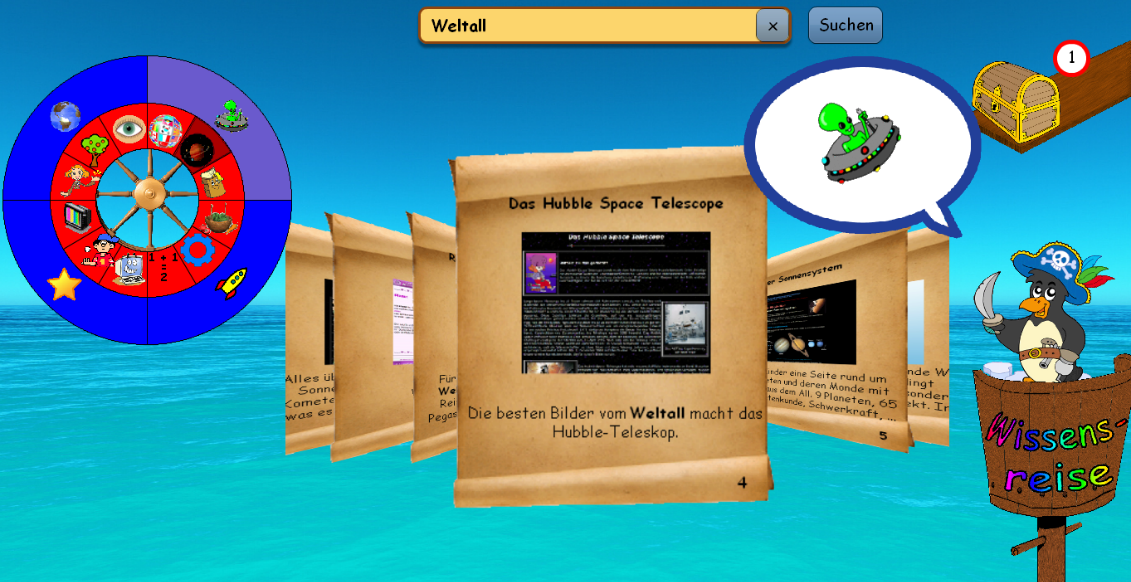
\includegraphics[width=1 \linewidth]{images/knowledge_journey.png}
    \caption{
        Knowledge Journey search interface \autocite[60]{gossen2012search}
    }
    %for reference to this figure
    \label{figure:KnowledgeJourney}
\end{figure}
Their interface presents information, which can also be retrieved with a conventional search engine, in a different way so that it is more inviting, interactable, and understandable for the minds of younger children. Furthermore, \textcite{gossen2012search} introduced a guidance character to handle possible failure and inexperience children may stumble upon.

Another case was introduced by \textcite{alhussayen2015evaluating}, where they launched an Arabic website called ``Aseel Wa Raseel'' that offers educational games for children. Although they used user-centered design in their development process, their platform revealed some troubles for younger children. On their website, \textcite{alhussayen2015evaluating} included a rather long registration process, that prevented all younger children (seven to nine years old) and the majority of the older ones (ten to twelve years) from registering on the website. 

\textcite{engen2017collaborative} conducted a study on an app that lets children create their own stories or fairy tales. In the study, the primary school children worked in groups to create a fairy tale and obtained a collaborative multimedia project at the of one week. Thus, the children gathered audio recordings, pictures, and texts during their process to accomplish their new self-made projects \autocite{engen2017collaborative}. \textcite{engen2017collaborative} concluded that the application was positively received since it is a very interactive and engaging tool. No child got excluded during the storytelling process, and every student could propose and include their ideas without any problems.
Furthermore, the children were able to focus on the application intensively and hence partake in a collective writing adventure \autocite{engen2017collaborative}.

\subsubsection{Augmented and Virtual Reality Applications}
Lastly, a rather innovative strategy is the implementation of augmented or virtual reality applications \autocite{saidin2015review, lozano2016dedigitalizing}. \\
Based on this strategy, \textcite{kerawalla2006making} analyzed different applications, including the solar system as the subject matter. These augmented reality applications were presented to children in elementary schools.
Although the children could create and manipulate the environment containing the planets, e.g., change size and rotation, it was mostly only animations to watch. Since the 3D animations did not require any further interaction, most children preferred simple role-play activities, where they could modify roles and interact with each other instead of only observe the 3D augmented animation \autocite{kerawalla2006making}.

Furthermore, \textcite{lozano2016dedigitalizing} introduced an educational game, that helps children build and refresh their knowledge of health literacy. With the help of tangible interfaces and mobile devices, \textcite{lozano2016dedigitalizing} succeeded to increase the motivation and satisfaction of the children. 

\textcite{saidin2015review} reviewed several different AR applications and concluded that AR has significant future potential, but still must be further developed. Most AR interfaces received positive feedback from the teacher side as well as from the student side. Especially the students proved to be more engaged with the learning process in schools \autocite{saidin2015review}.

Interactive and augmented applications also establish a multi-sensory learning approach, which furthermore promotes a conducive learning process in schools \autocite{cabero2016educational}. Aside from sight and therefore the visual content, AR implementations also offer additional stimulus for touch and hearing, for example in videos \autocite{saidin2015review, cabero2016educational, lozano2016dedigitalizing}. Through the integration of touching elements, hence with the help of tangible interfaces, children are able to gain several skills and overall notably benefit from technology \autocite{saidin2015review, cabero2016educational}. Furthermore, children experience a more familiar and reality-based interaction, and it feels more natural to them, which is especially important for younger children \autocite{lozano2016dedigitalizing}.

\subsection{Why Children need different interfaces}
\label{subsection:ChildrenInterfaces}
Technology has been evolving over the last decades \autocite{walker2000screen}. Hence, the majority of the popularity that has access to these high-tech appliances has integrated technology into their daily lives \autocite{sharmin2012effect, walker2000screen}. As a result, children have become used to technology and already have prior knowledge \autocite{walker2000screen, gikas2013mobile}. When children get introduced to new technology, e.g., in school, they process the newly discovered information differently in comparison to adults \autocite{gossen2012search}. \\
As \textcite{alhussayen2015evaluating} disclose in their paper, children approach situations and their surroundings differently. That is because the physical, as well as the cognitive abilities and skills of the children, are not fully developed yet. Until they reach adulthood, their interests and also their developmental needs differ from those of a grown-up \autocite{gossen2012search, alhussayen2015evaluating}. As a consequence, interfaces for children need to be adapted to their abilities, interests, and needs as \textcite{gossen2012search} emphasize in their paper.

\textcite{kermani2015preparing} found in their study, which is about an unconventional way of integrating science and math into the daily curriculum in school, that children tend to favor topics that are already familiar to them. Consequently, children prefer popular topics but appreciate the possibility for the expansion of potential unfamiliar factors. \textcite{kermani2015preparing} observe in their study, that this combination is the basis for humans to establish adequate long-term knowledge about new topics presented to them as children.

Moreover, children have not yet developed their reading skills as well as adults and therefore have different, and from child to child varying, reading patterns. Thus, reading time decreases when age increases \autocite{sharmin2012effect, adattil2018effects}. Furthermore, \textcite{adattil2018effects} focus on typography, which plays a fairly significant role when it comes to the reading ability of children. Since students prefer e-resources over hard copies, there are more factors than only font size that result in optimal reading material \autocite{adattil2018effects}. \textcite{adattil2018effects} deduced that in electronic reading material, change of brightness, the overall composition of the text and font color could change the readability of a text.\\
In their study, \textcite{sharmin2012effect} detected specific reading preferences while looking at the eye movements of the children that participated in their study. \textcite{sharmin2012effect} compared the eye movements of the children while reading paragraphs, sentences, lines, and only word chunks. They concluded that children tended to have shorter fixation duration on longer paragraphs or sentences. Hence, the eye movements were smoother, and it was easier to read for the children \autocite{sharmin2012effect}. In contrast to fairly long texts, word chunks and individual lines received more fixations, because the eyes had to concentrate on only one point \autocite{sharmin2012effect}. \textcite{sharmin2012effect} concluded, that longer paragraphs in texts are easier to read and therefore confirmed the findings of prior studies and approaches.

In the course of their study, \textcite{gossen2012search} implemented a search engine called ``Knowledge Journey'' for primary school children. During this implementation, they suggested not to disregard that children need additional support on regular websites and applications. Overall, they mentioned six types: emotional, language, cognitive, memory, interaction, and relevance support \autocite{gossen2012search}. \\
Firstly, they proposed inserting a guidance character to handle any errors and emotionally support the child, so a feeling of success will persist \autocite{gossen2012search}.\\
Secondly, since children are still developing their reading and writing abilities, the search should not be limited to text-based information only. For example, the integration of images and audio help can assist their additional need for language support \autocite{gossen2012search}.\\
Thirdly, \textcite{gossen2012search} note that children in primary school are still cognitively developing. As a consequence, all icons and possibly used metaphors should always have a direct and definite relation to reality. \\
Fourth, children need supplementary memory support because it is not fully developed either. In order not to overwhelm a child with information, the presented data on a website must be limited \autocite{gossen2012search}. Furthermore, children tend to look at the same thing more often than adults \autocite{gossen2012search}. To support that, \textcite{gossen2012search} suggested integrating some sort of storage possibility, so that a child can always revisit the saved information.\\
Fifth, the fine motor skills of a child are not as advanced, which may reduce interaction with an interface. As a result, all clickable items on a website should be big enough and no too complicated operations like scrolling should be integrated \autocite{gossen2012search}.\\
Lastly, children need help deciding whether or not the information is relevant. Hence, the data should always be presented well-ordered. For their search engine, they also introduced horizontal navigation for the results, where each item had an image attached to the text \autocite{gossen2012search}.

To sum up, the research from all the studies showed that children indeed need different interfaces for various vital reasons \autocite{sharmin2012effect, gossen2012search, kermani2015preparing, adattil2018effects}.

\section{Practical Part}
\label{section:PracticalPart}
In the course of this thesis, a study has been conducted to solidify all the findings collected in regards to designing interfaces that are specifically made for children. As \textcite{gossen2012search, engen2014ipads, lozano2016dedigitalizing} mention in their papers, it is necessary to devise different interfaces for children in comparison to interfaces made for adults. Furthermore, it is essential to include the children's needs and interests in the designing process.\\
Subsequently, the following sub-chapters will disclose how the prototype got implemented and tested with twenty-two school primary children. Additionally, all new findings and results of the user study will be accurately analyzed and further evaluated in the following sections. 

\subsection{Implementing the prototype}
\label{subsection:ImplementingPrototype}
For the implementation of this thesis, a React\footnote{https://reactjs.org/} project has been developed. As previous research results by \textcite{gossen2012search, lozano2016dedigitalizing} showed, gamified and rather interactive approaches turned out to be more preferred by elementary school children. For this reason, the study conducted for this paper too introduces an interactive application in the form of a quiz about health literacy (see Figure \ref{figure:QuizHome} for the home screen of the quiz). 
\begin{figure}[!ht]
    \centering
    \includegraphics[width=1 \linewidth]{images/quiz_home.png}
    \caption{
        The home screen of the implemented quiz specifically designed for children
    }
    \label{figure:QuizHome}
\end{figure}
As a result, the following sections will include an explanation about the health literacy content for the prototype, and how information was chosen and collected. Furthermore, the general composition of this quiz application will be accurately described.

\subsubsection{Content}
Since health literacy is constantly a part of our daily lives, it is the chosen topic for this application. Furthermore, as \textcite{velardo2017emphasizing} emphasize in their paper, it is important to introduce the concept of health literacy at an early age and adapt the delivery of the content so that children can process the given information accurately. \\
Practical knowledge, for example, hygiene or daily routines as \textcite{paakkari2012health} describe in their paper, is most familiar to children. Therefore, the focus of the topic presented in this prototype is on nutrition. To adapt the information optimally to the abilities and needs of children, the contents that were chosen for this prototype were adapted from child-appropriate websites and online quizzes about health literacy. 
For example, the content of one question about dental hygiene was adjusted from the \textcite{junior2019teeth} website. The question about the sugar content in beverages was compiled knowledge based on the information collected from the article ``10 Fragen zu Zucker und Coca-Cola'' from the Swiss Coca-Cola website \autocite{cola2017sugar}. Aside from that, the remaining content was gathered and accommodated from other various health-related web quizzes. These different websites were also particularly constructed for younger minds with the intention to be viewed by primarily elementary school children \autocite{swr2019nutrition, junior2019vitamins}. 
Although the quiz was made to inform children about health literacy and improve their knowledge on a long-term basis, all questions displayed in the prototype of this study are suggestions. As a result, these recommendations may serve as a guide but must not be taken as ground rules.

Nonetheless, the following seven questions were generated to test the children's knowledge about health literacy. 
\begin{enumerate}
    \item Which of the following food items is the best for you and therefore you could eat them every day?
    \begin{enumerate}
        \item Chocolate and other sweets
        \item Burger and fries
        \item Fruits and vegetables
        \item Pizza
    \end{enumerate}
    \item How many sugar cubes are in a normal 250ml glass filled with Coca-Cola? (Drag the correct number of cubes into the answer area)
    \item A one-sided diet (always burger or only eating sweets) is very healthy.
    \begin{enumerate}
        \item True, only eating chocolate and burgers is totally healthy
        \item False, you should eat a diversified diet and not forget about fruits and vegetables
    \end{enumerate}
    \item How often should you brush your teeth?
    \begin{enumerate}
        \item Once a week is enough
        \item Every other day
        \item Never
        \item Two to three times a day, always after a meal
    \end{enumerate}
    \item In order to help the brain with its work, we can eat vitamins in the form of fruits and vegetables. Is that correct? 
    \begin{enumerate}
        \item No, vitamins do not help, but greasy food like fries helps with that.
        \item Yes. Especially the vitamins A, C and E help our brain to work.
    \end{enumerate}
    \item Match the food to the corresponding baskets below. (Apple, carrot, sweets, donuts, hot dog)
    \begin{enumerate}
        \item Basket 1: This is very good, and you can eat it every day
        \item Basket 2: There is no problem if you eat this every now and then
        \item Basket 3: You should not eat that often or not at all
    \end{enumerate}
    \item What is the best thing for your body and keeps you fit?
    \begin{enumerate}
        \item Sitting at home while only reading 
        \item Playing outside with friends or riding a bike
        \item Playing computer games at home all day 
        \item Being lazy, lying around and watching television the whole day day
    \end{enumerate}
\end{enumerate}

\subsubsection{Composition of the prototype}
The realized prototype for this study has the purpose of being particularly appealing to children. Since \textcite{sharmin2012effect} discovered in their study, that children prefer reading lengthier texts in comparison to short sentences and word chunks, the attempt in this prototype was also not to phrase questions and texts that are too short.
To further adapt the visual design to the needs of children, the typography was adjusted as well \autocite{adattil2018effects}.
Moreover, for the distinct reason for being engaging for children, there have been introduced four different ways in which the seven included questions are sculpted to make the application more engaging.

Firstly, there are three multiple-choice questions, where each question has four possible options to choose an answer from. Additionally, every answer has an image included (see Figure \ref{subfigure:QuizMultipleChoice}) to make the application more engaging and to adapt it further to the interests and needs of children. \\
Secondly, the app also includes two true or false questions. Similar to the multiple-choice questions, this type also contains a topic-related picture to make it more appealing to the eyes (see Figure \ref{subfigure:QuizTrueFalse}).\\
Thirdly, there is one question about the sugar content in beverages. To answer this question, the children needed to drag the corresponding amount of sugar cubes, which are included in a specific drink, into the grey answer area (see Figure \ref{subfigure:QuizCubes}).\\
Lastly, there is another question about different types of food that needs to be sorted into the corresponding categories. These categories (in the form of three baskets - see Figure \ref{subfigure:QuizAssign}) have been classified based on how healthy the varying foods are for humans and how often one should eat them to maintain proper health. 
\begin{figure}[!ht]
    \centering
    \subfloat[Multiple-choice questions with four possible answers]{
        \includegraphics[width=0.45\linewidth]{images/quiz_multiple_choice.png}
        \label{subfigure:QuizMultipleChoice}
    }
    \qquad
    \subfloat[True or false options]{
        \includegraphics[width=0.45\linewidth]{images/quiz_true_false.png}
        \label{subfigure:QuizTrueFalse}
    }
    \caption[
        Different types of simple questions included in the quiz %\newline
        % source url given in the table of figures
        %\small\texttt{https://mytestproject-2018.firebaseapp.com/}
    ]{
        Different types of questions that are included in the quiz
    }
    %for reference to all subfigures
    \label{figure:QuizQuestions}
\end{figure}

\begin{figure}[!ht]
    \centering
    \subfloat[Guessing the sugar content in beverages]{
        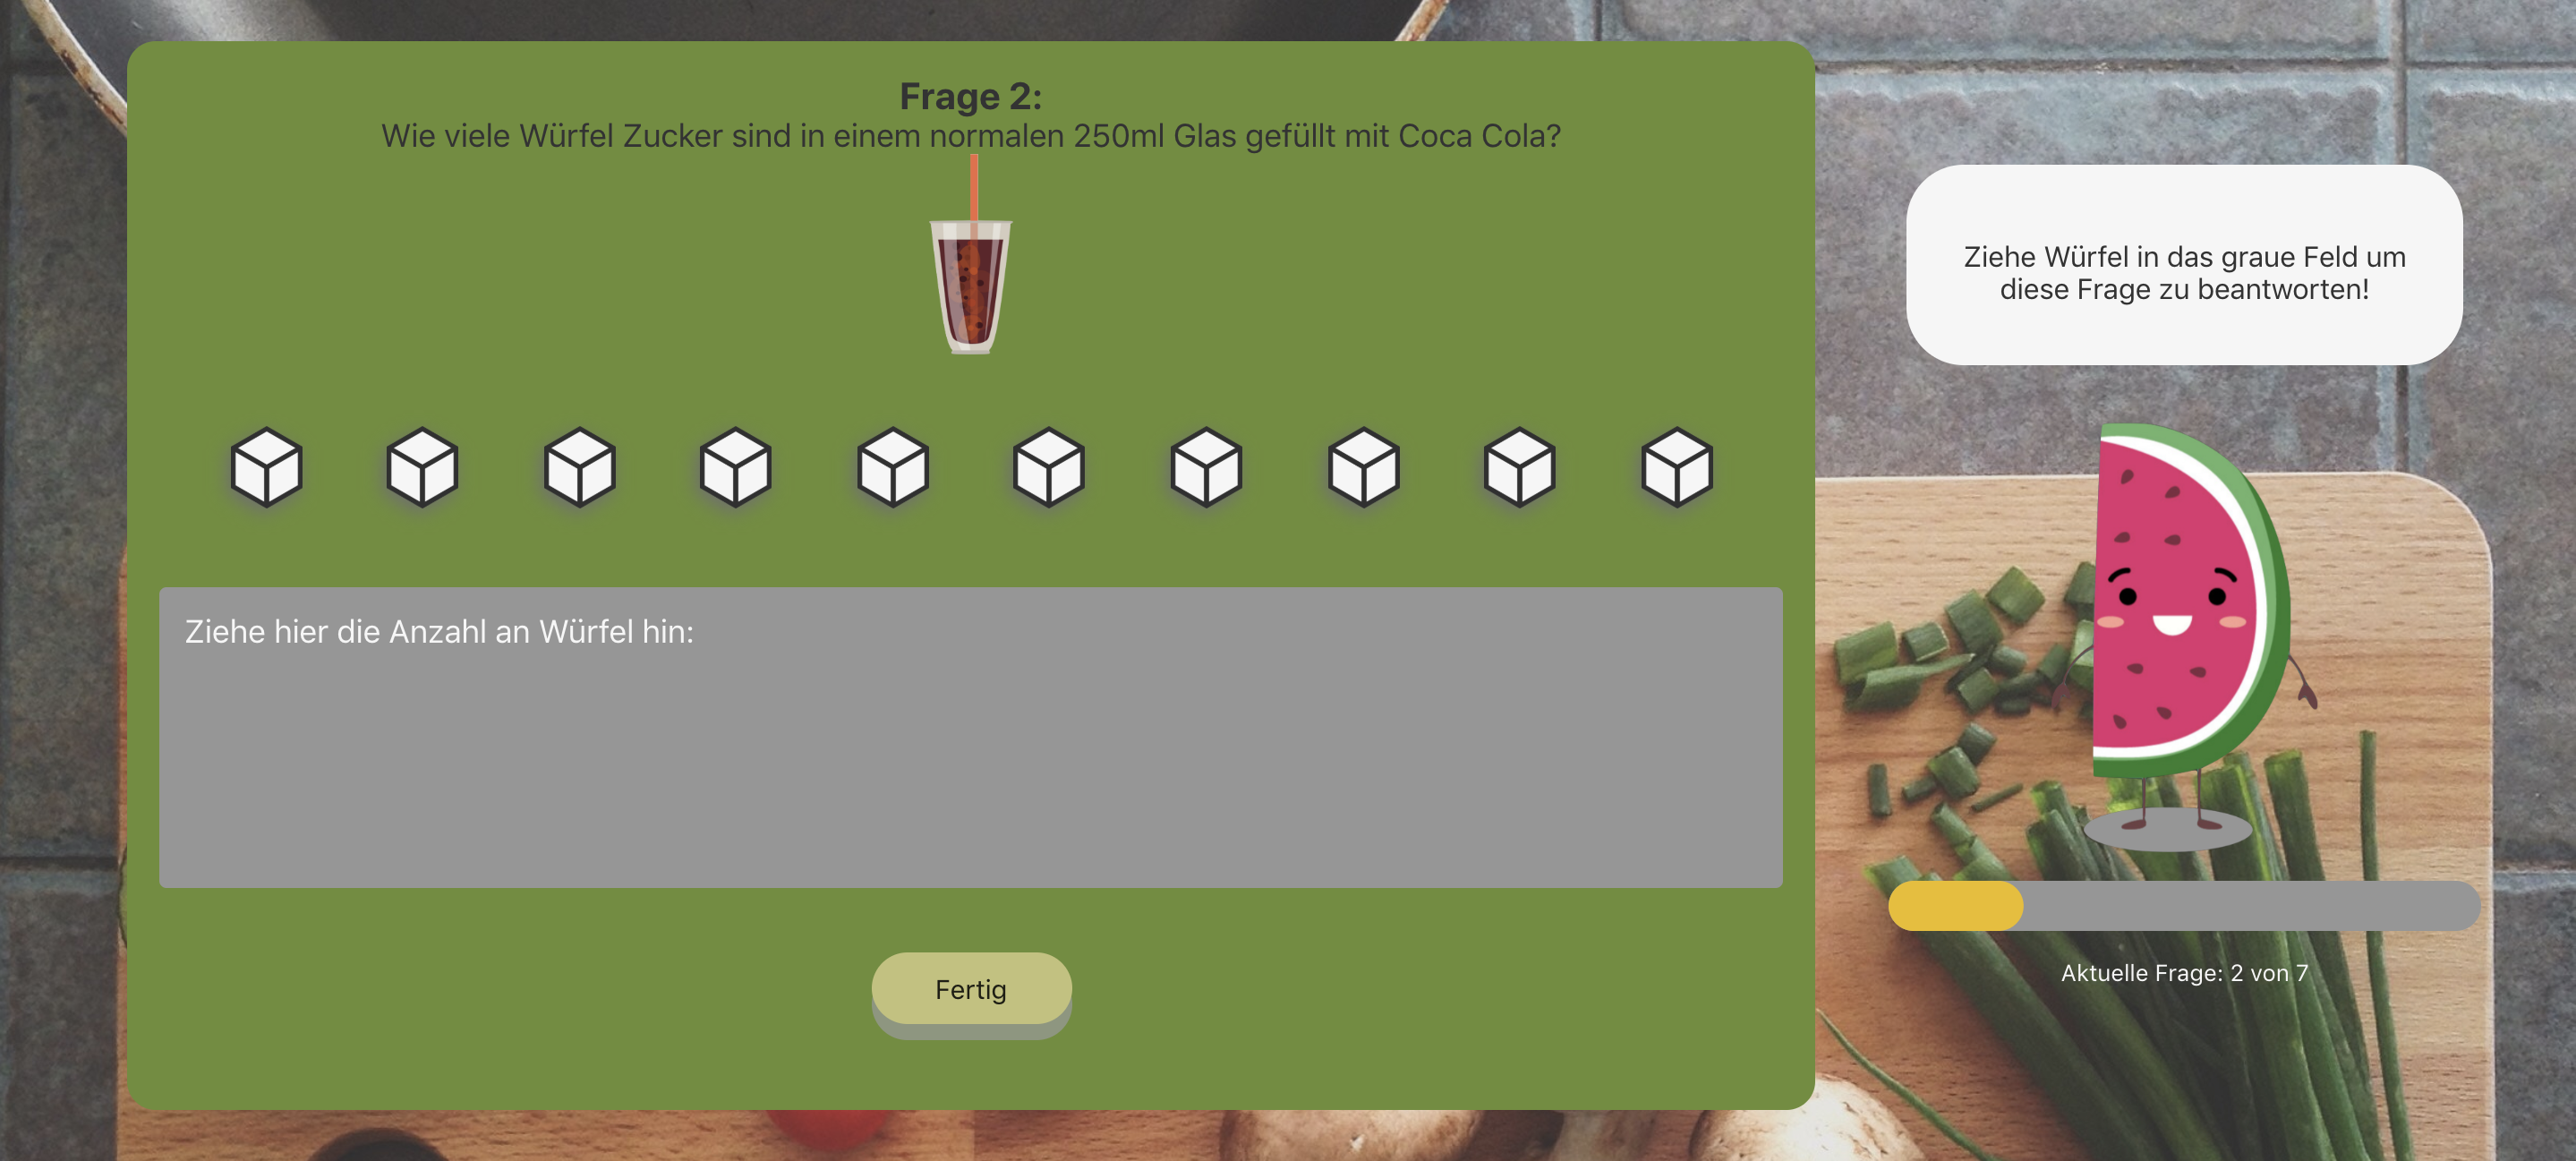
\includegraphics[width=0.97\linewidth]{images/quiz_cubes.png}
        \label{subfigure:QuizCubes}
    }
    \qquad
    \subfloat[Assigning food to the correct categories]{
        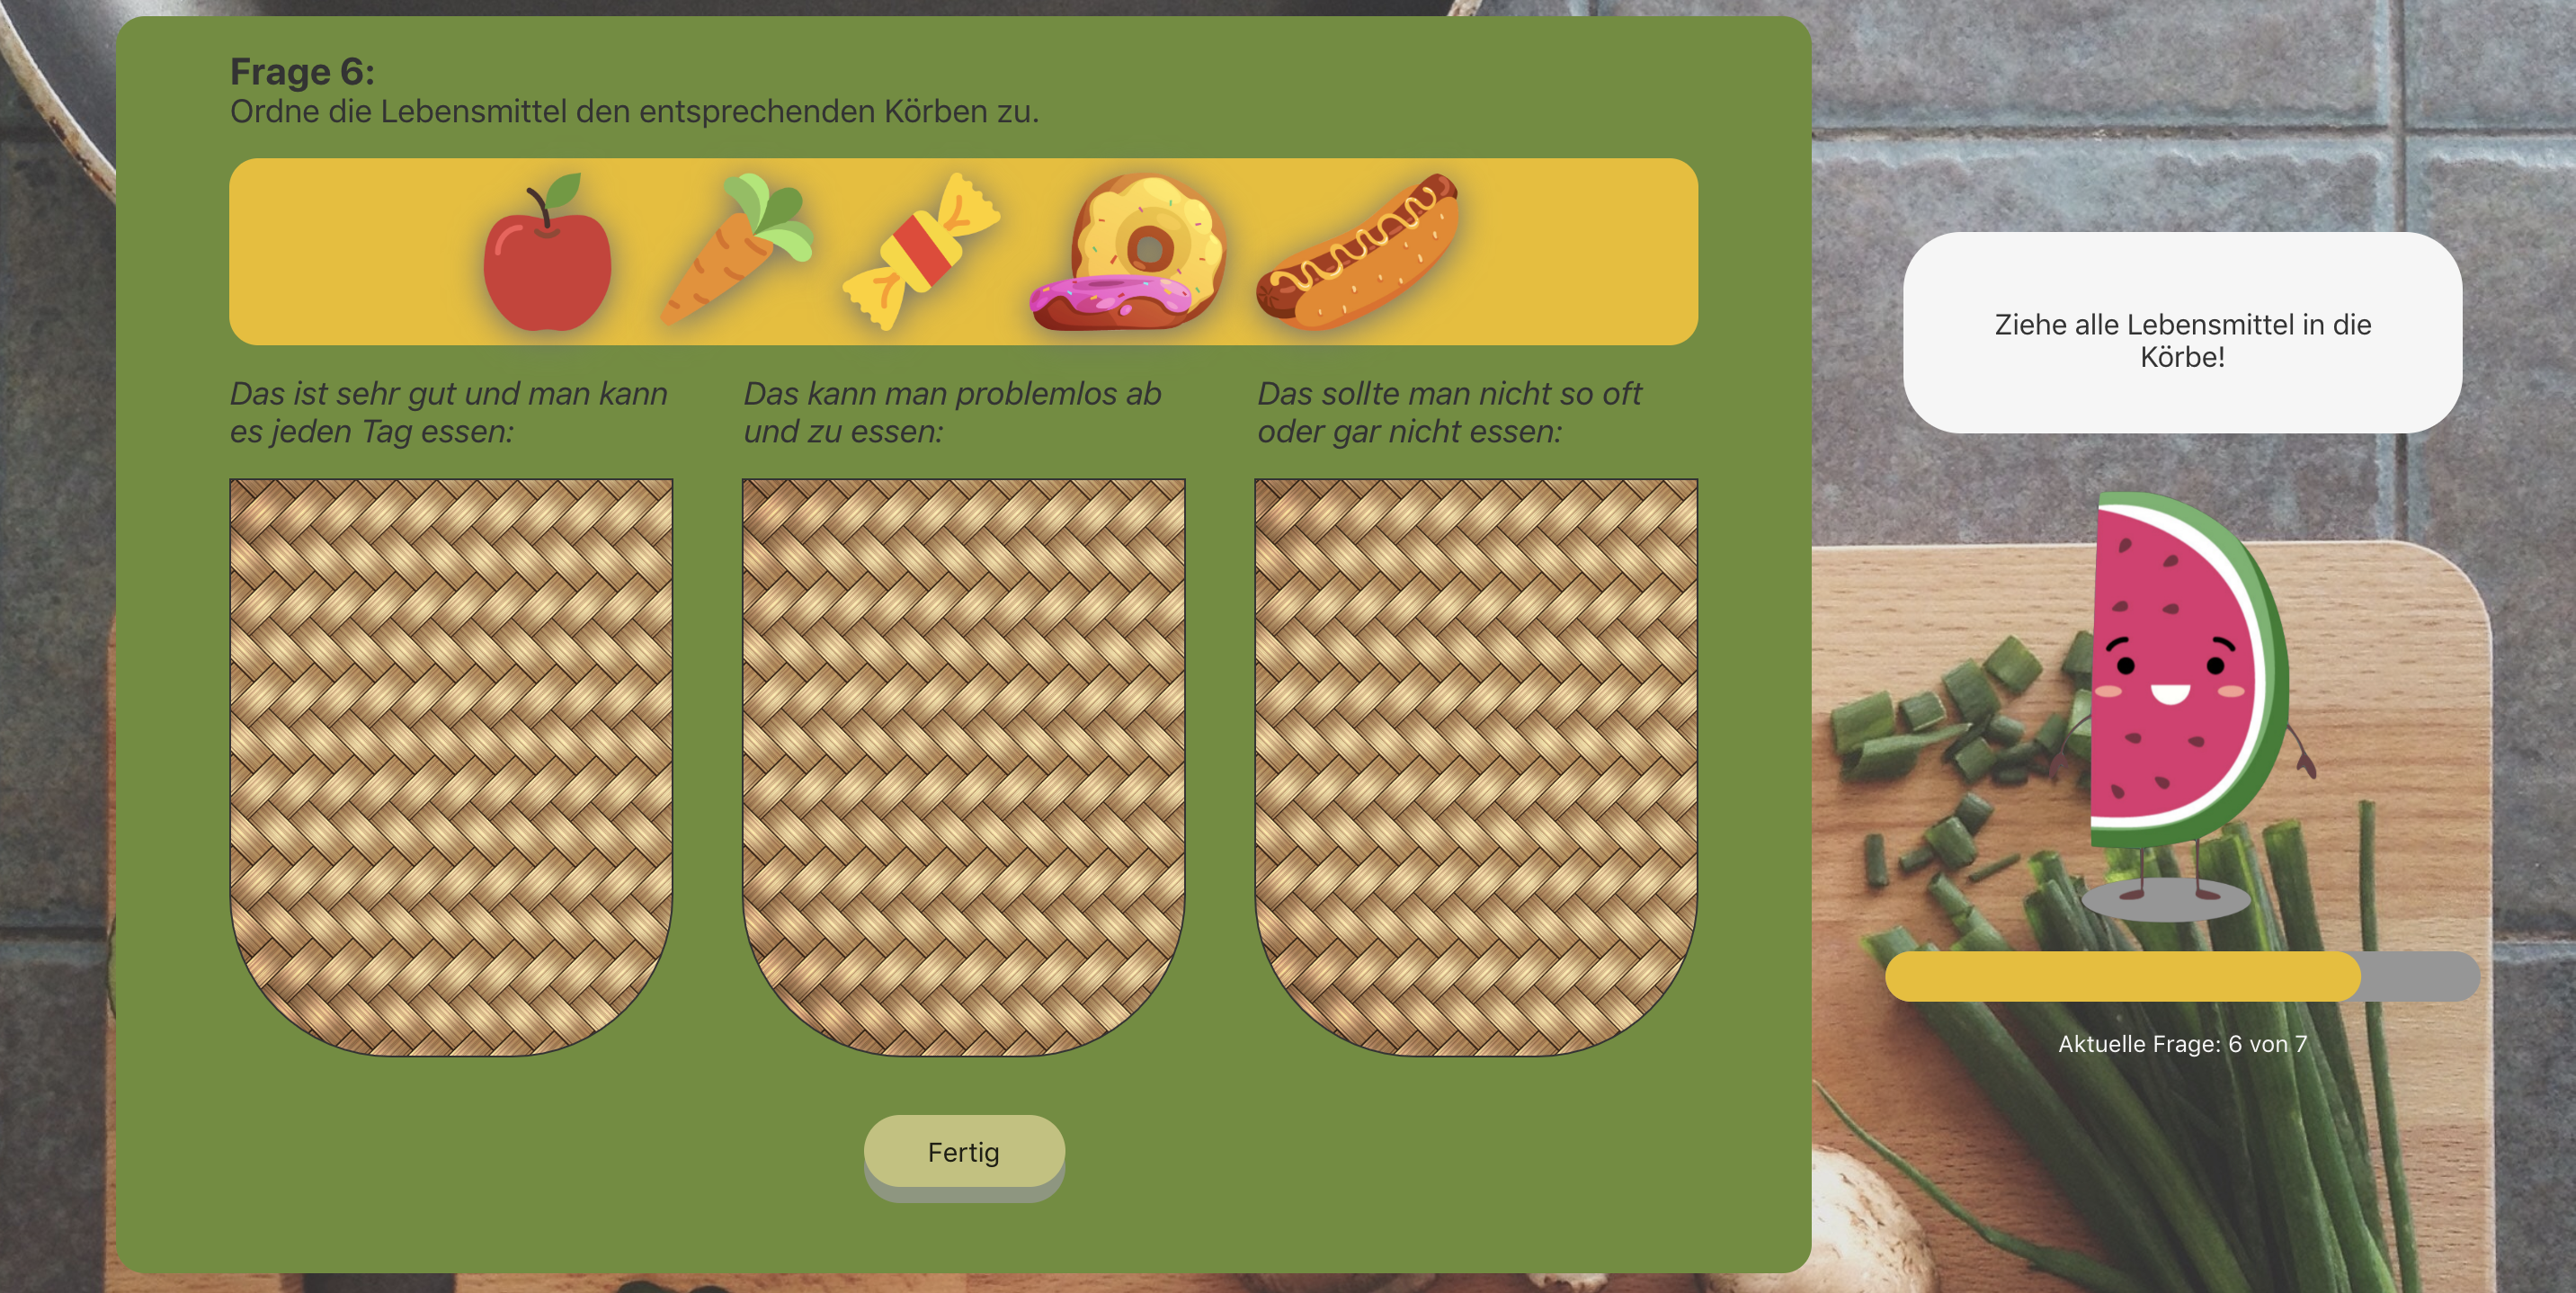
\includegraphics[width=0.97\linewidth]{images/quiz_assign.png}
        \label{subfigure:QuizAssign}
    }
    \caption[
        Different types of questions included in the quiz %\newline
        % source url given in the table of figures
        %\small\texttt{https://mytestproject-2018.firebaseapp.com/}
    ]{
        Two additional approaches to formulate a question
    }
    %for reference to all subfigures
    \label{figure:QuizQuestions2}
\end{figure}

Aside from the selection of different question types, there has additionally been introduced a guidance character. As mentioned before, the idea of some variety of guidance in the form of an approachable and more humanized character has already been introduced by \textcite{gossen2012search}. The character may help the children deal with any kind of errors and suggests further possible steps if the children do not know how to continue their search journey \autocite{gossen2012search}. For the prototype of this study, a humanized image of a watermelon has been chosen as the guidance character, which is also called the helper. Since the goal of this application is to inform and educate children about health and wholesome nutrition, a food item was deliberately selected to represent the humanized helper. 
Furthermore, the primary purpose of the helper is to display messages for the user and to handle any potential faults or errors. As a result, it offers visual and colored feedback (see Figure \ref{figure:HelperFeedback}) to make it easier for children to understand all presented commands. \\
\begin{figure}[!ht]
    \centering
    \subfloat[Colored warning feedback if a user manufactures a minor fault]{
        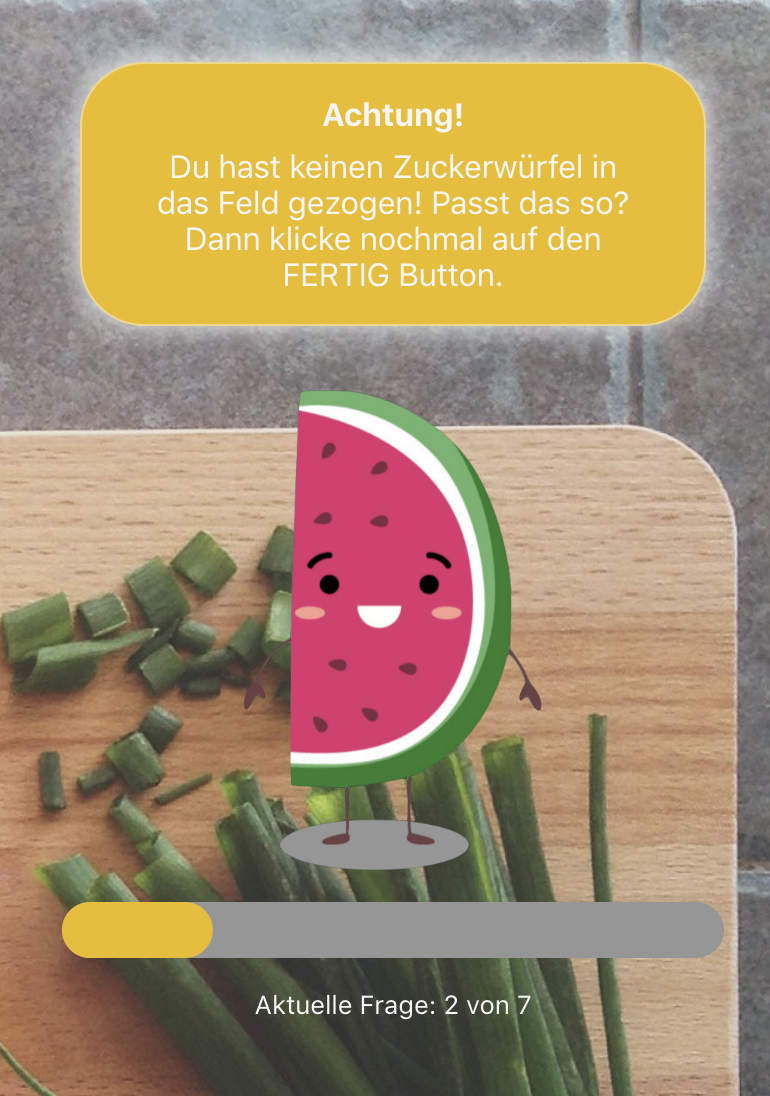
\includegraphics[width=0.4\linewidth]{images/helper_warning.png}
        \label{subfigure:HelperWarning}
    }
    \qquad
    \subfloat[Helper offers feedback if user answers question correctly]{
        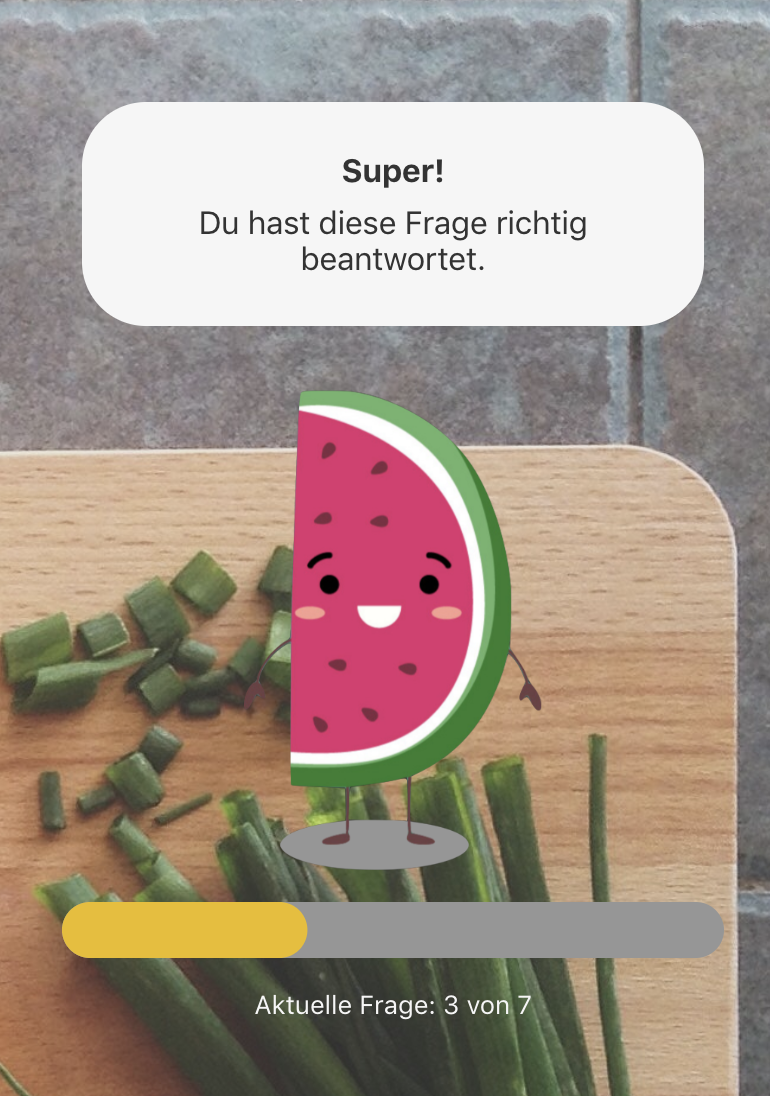
\includegraphics[width=0.4\linewidth]{images/helper_answer_correct.png}
        \label{subfigure:HelperAnswerCorrect}
    }
    \qquad
    \subfloat[Colored error feedback if a user input error occurs]{
        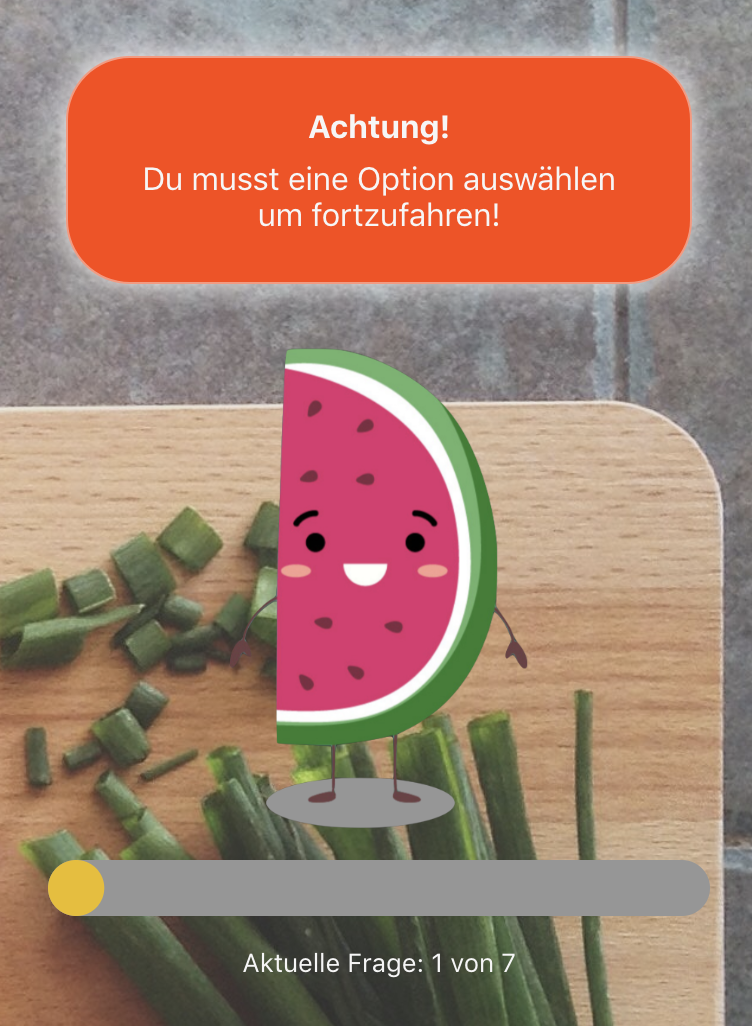
\includegraphics[width=0.4\linewidth]{images/helper_error.png}
        \label{subfigure:HelperError}
    }
    \qquad
    \subfloat[Guidance character displays feedback if answer is wrong]{
        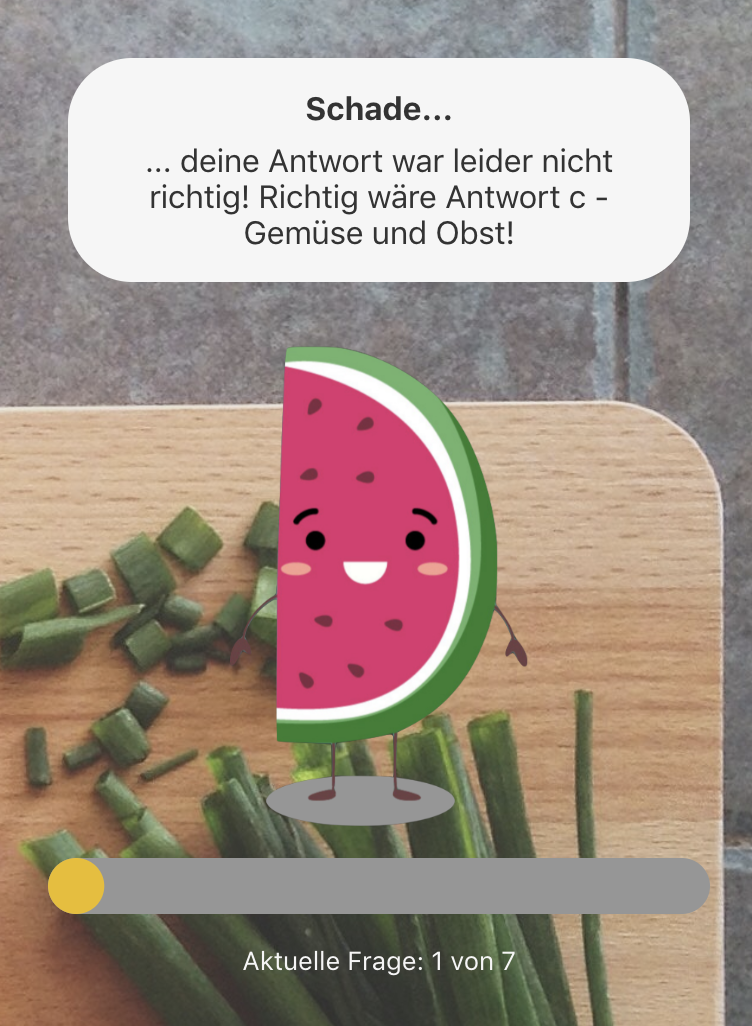
\includegraphics[width=0.4\linewidth]{images/helper_answer_wrong.png}
        \label{subfigure:HelperAnswerWrong}
    }
    \caption[
        Visual feedback that children receive from the guidance character  %\newline
        % source url given in the table of figures
        %\small\texttt{https://mytestproject-2018.firebaseapp.com/}
    ]{
        Visual feedback that children receive from the guidance character
    }
    %for reference to all subfigures
    \label{figure:HelperFeedback}
\end{figure}
Additionally, there is more visual feedback integrated to customize the interface as affable as possible for children. For example, if the current question is either multiple-choice or true or false, the given answer gets immediately evaluated. As a consequence, to provide a well cognizable assessment, a correct given answer is highlighted green and a wrong one accordingly red as presented in Figure \ref{figure:Answers}.\\
\begin{figure}[!ht]
    \centering
    \subfloat[Question correctly answered with immediate feedback]{
        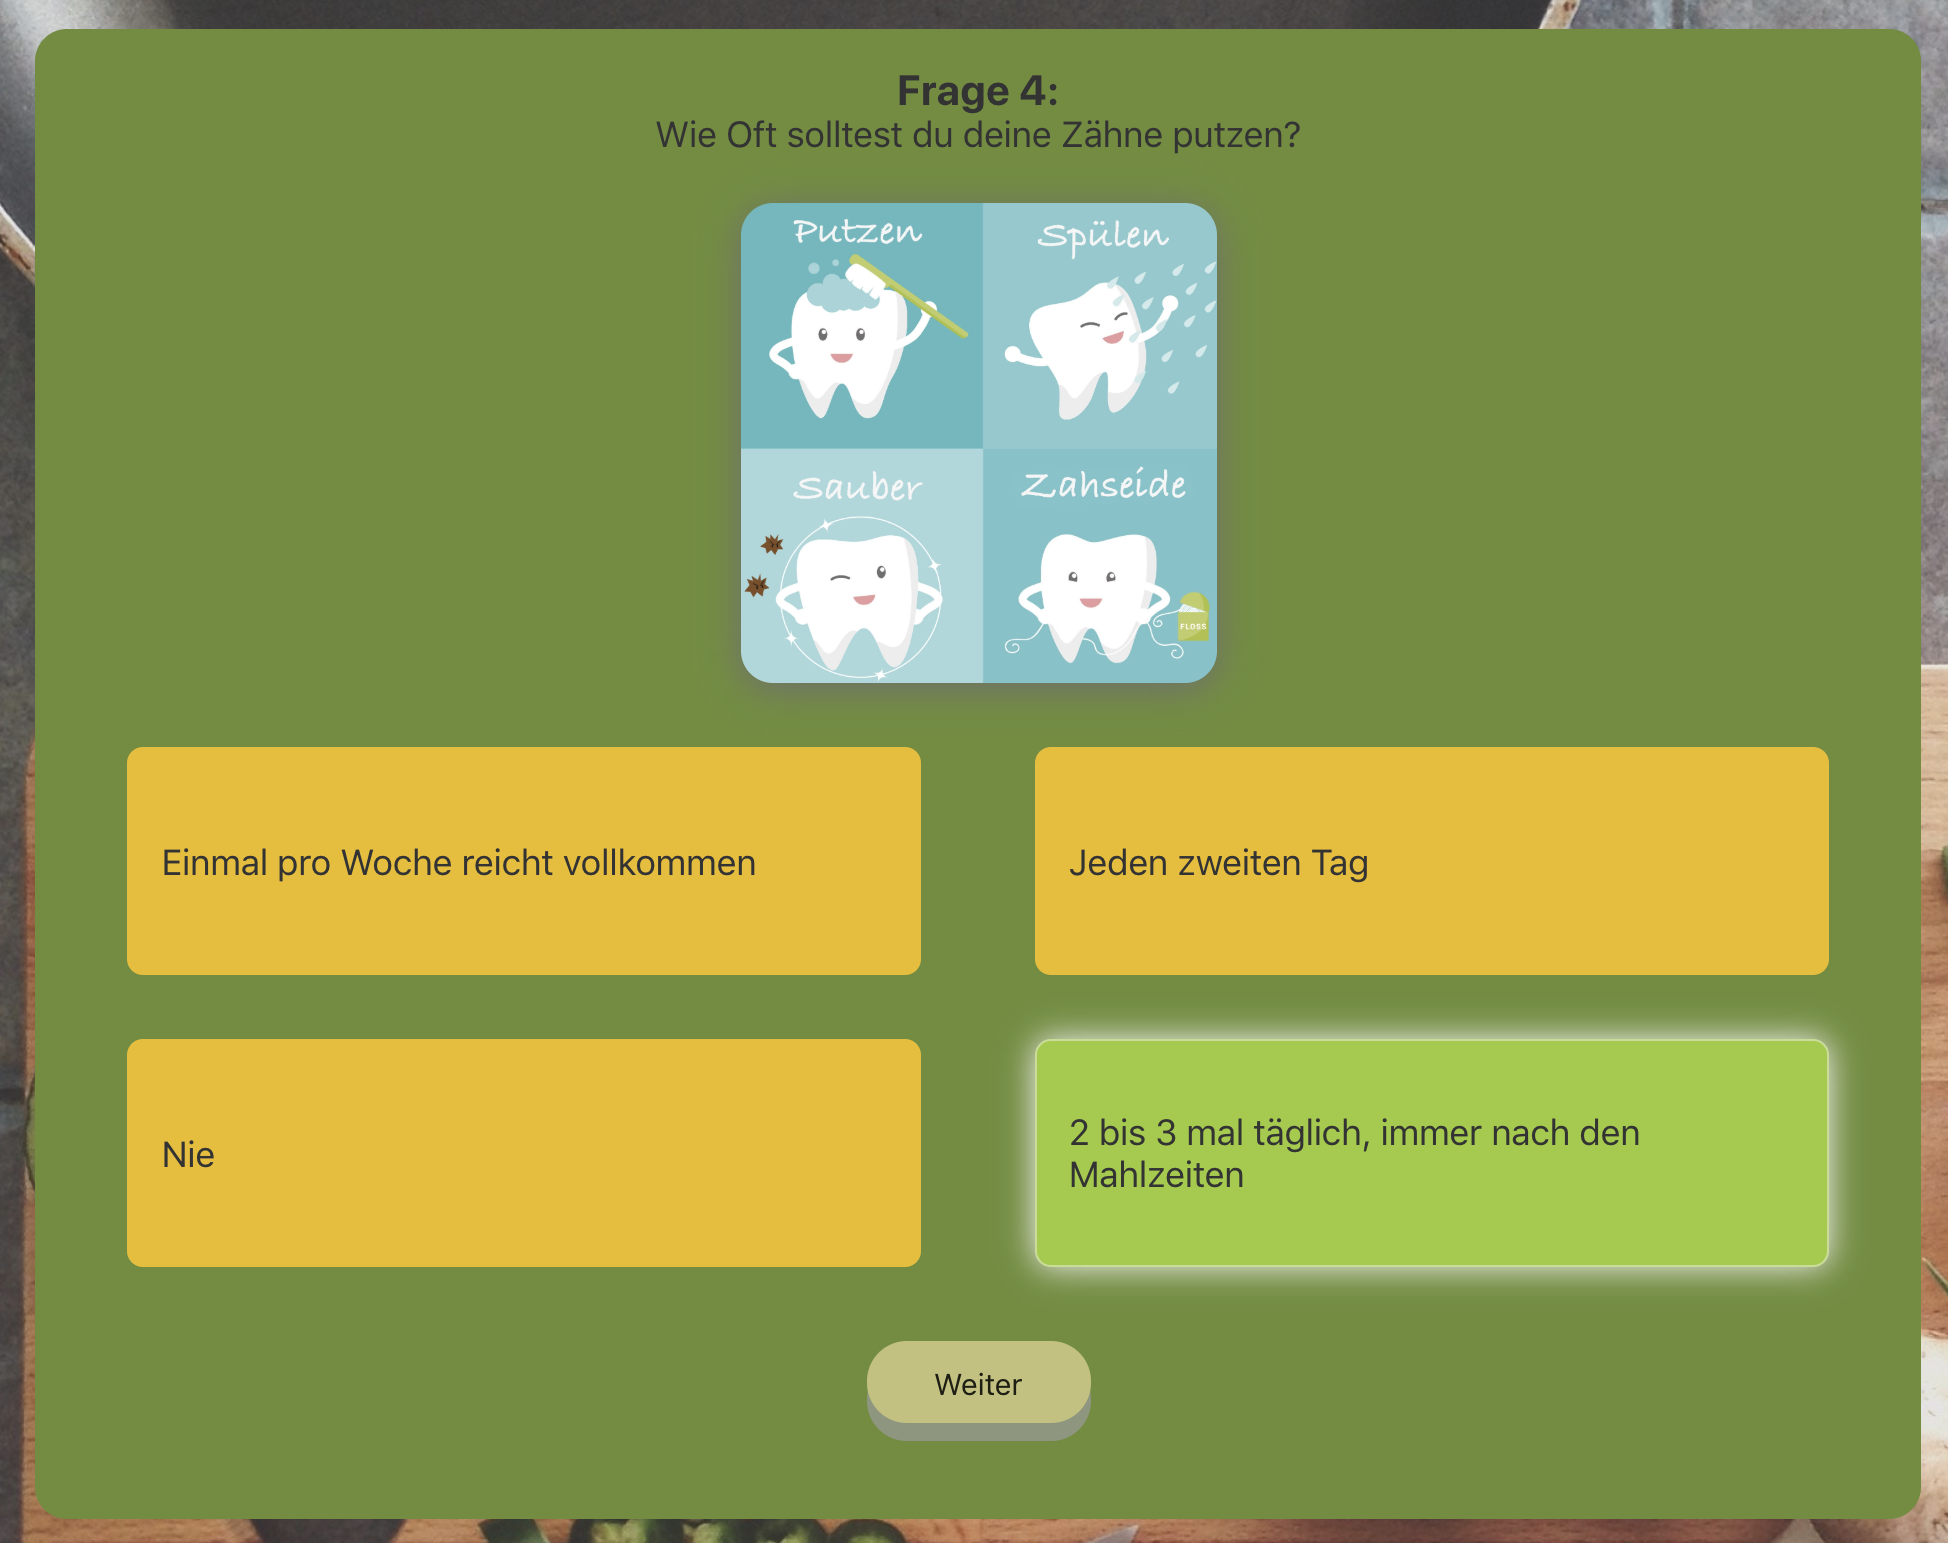
\includegraphics[width=0.45\linewidth]{images/answers_correct.png}
        \label{subfigure:AnswersCorrect}
    }
    \qquad
    \subfloat[Question not answered correctly]{
        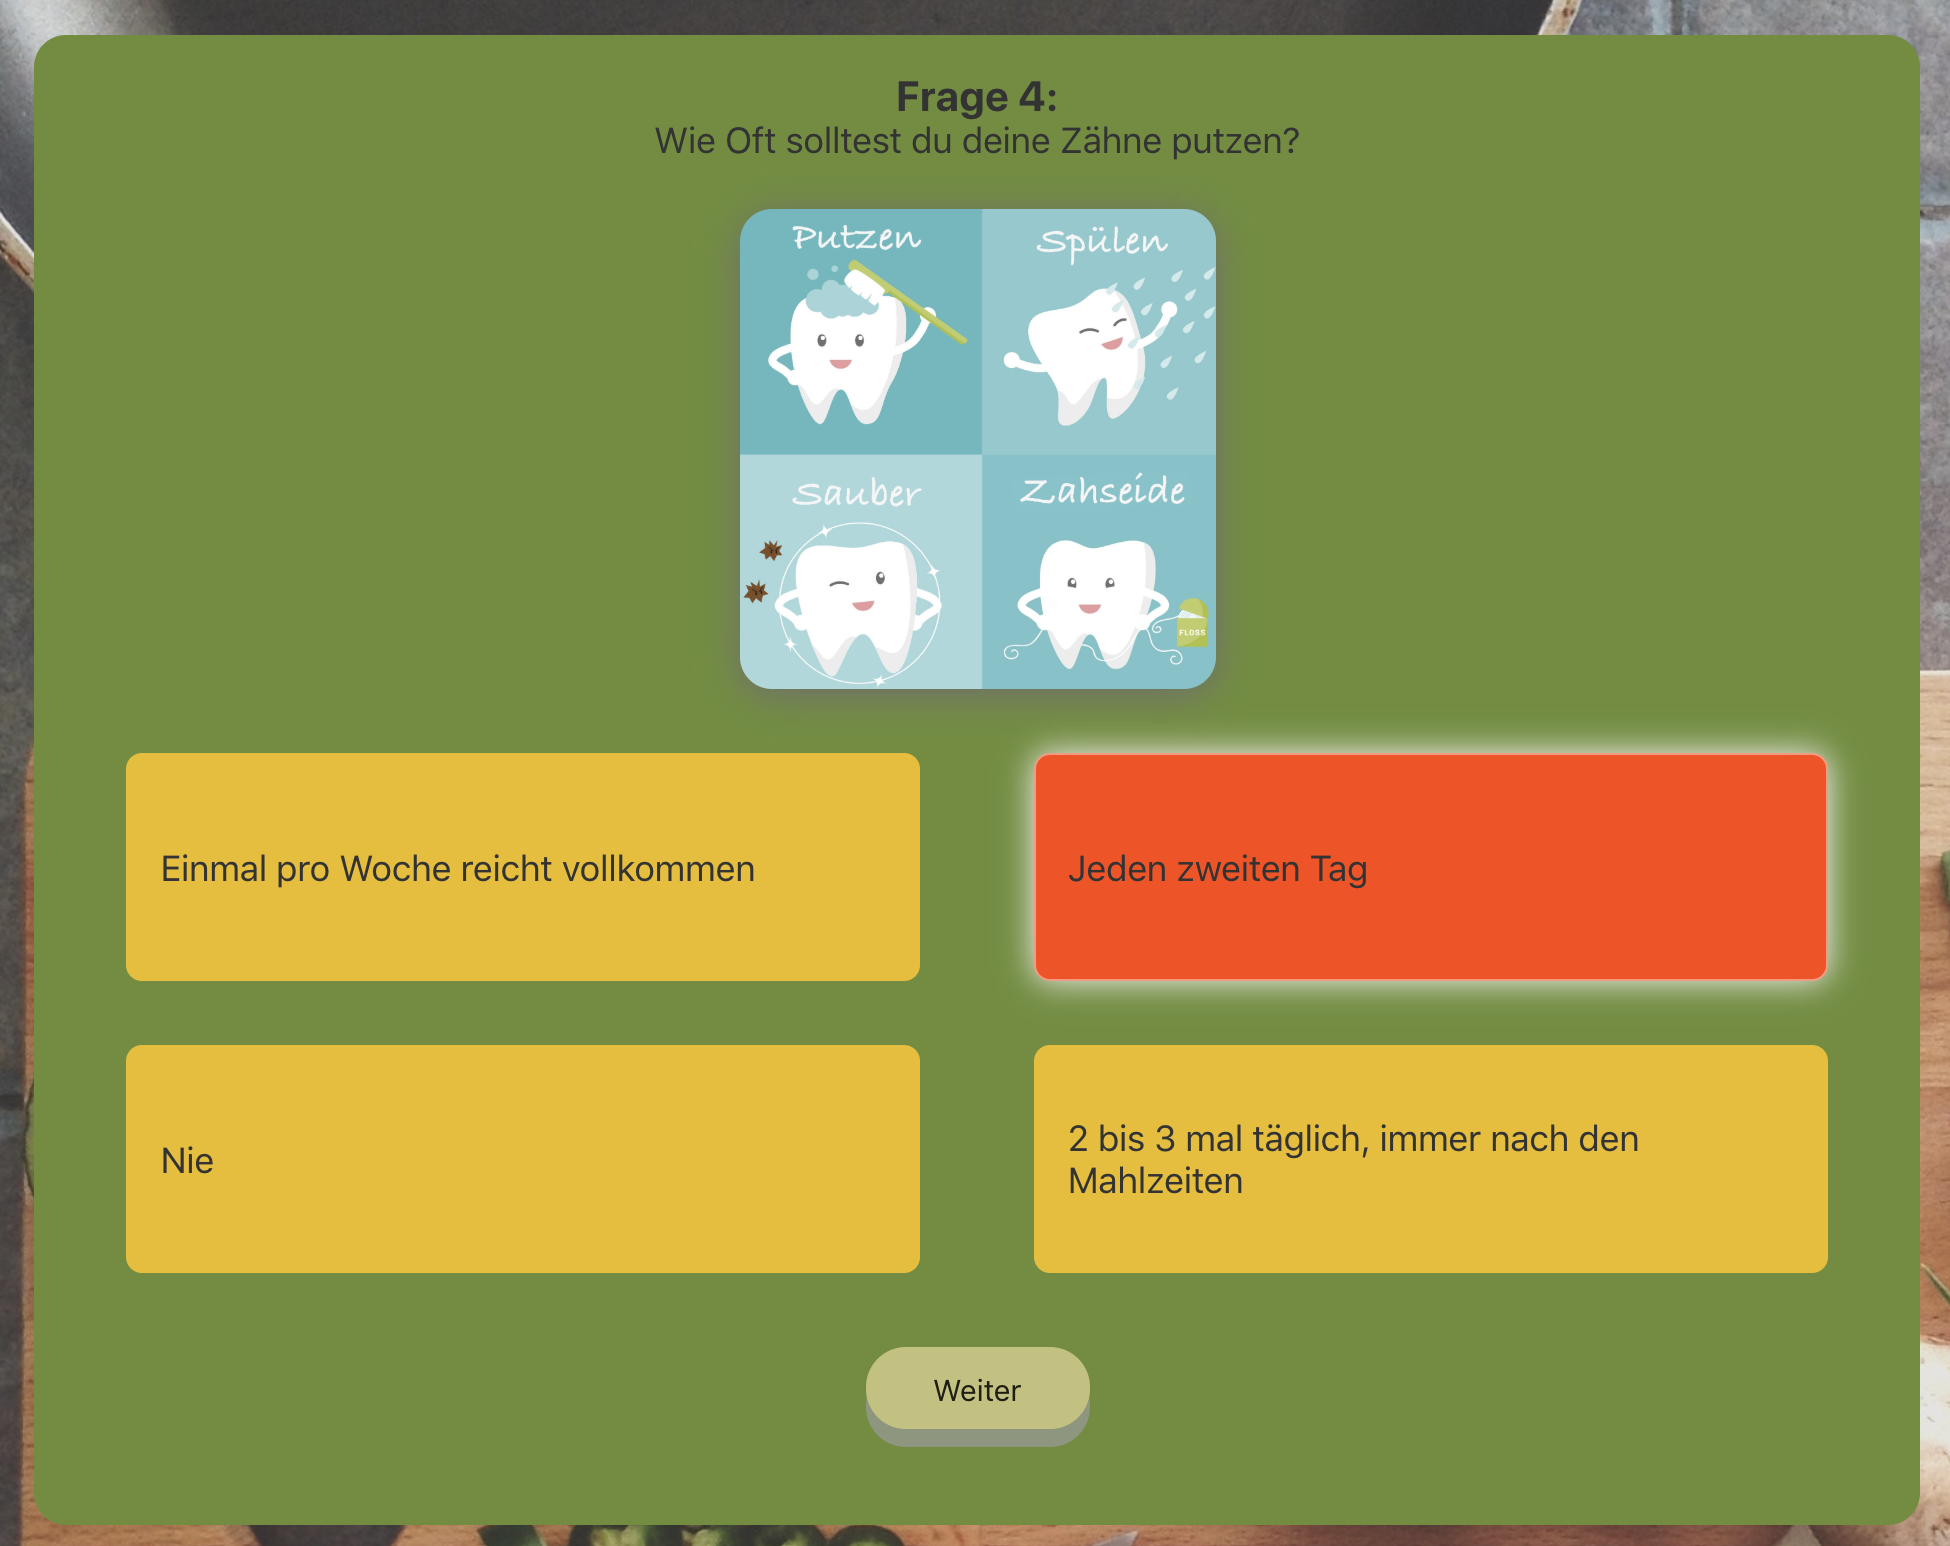
\includegraphics[width=0.45\linewidth]{images/answers_wrong.png}
        \label{subfigure:AnswersWrong}
    }
    \caption[
        Visual feedback for either correct or false given answer for multiple-choice question %\newline
        % source url given in the table of figures
        %\small\texttt{https://mytestproject-2018.firebaseapp.com/}
    ]{
        Visual feedback for either correct or false given answer for multiple-choice question
    }
    %for reference to all subfigures
    \label{figure:Answers}
\end{figure}

Moreover, the quiz application also contains a comprehensive evaluation on the finish-screen at the end of the quiz. Consequently, after exercising their knowledge about health literacy via the quiz, the child is either simply satisfied with the number of their correct answers or they can then review their complete scores and further evaluation by pressing the affiliated link (see Figure \ref{figure:Evaluation}).
\begin{figure}[!ht]
    \centering
    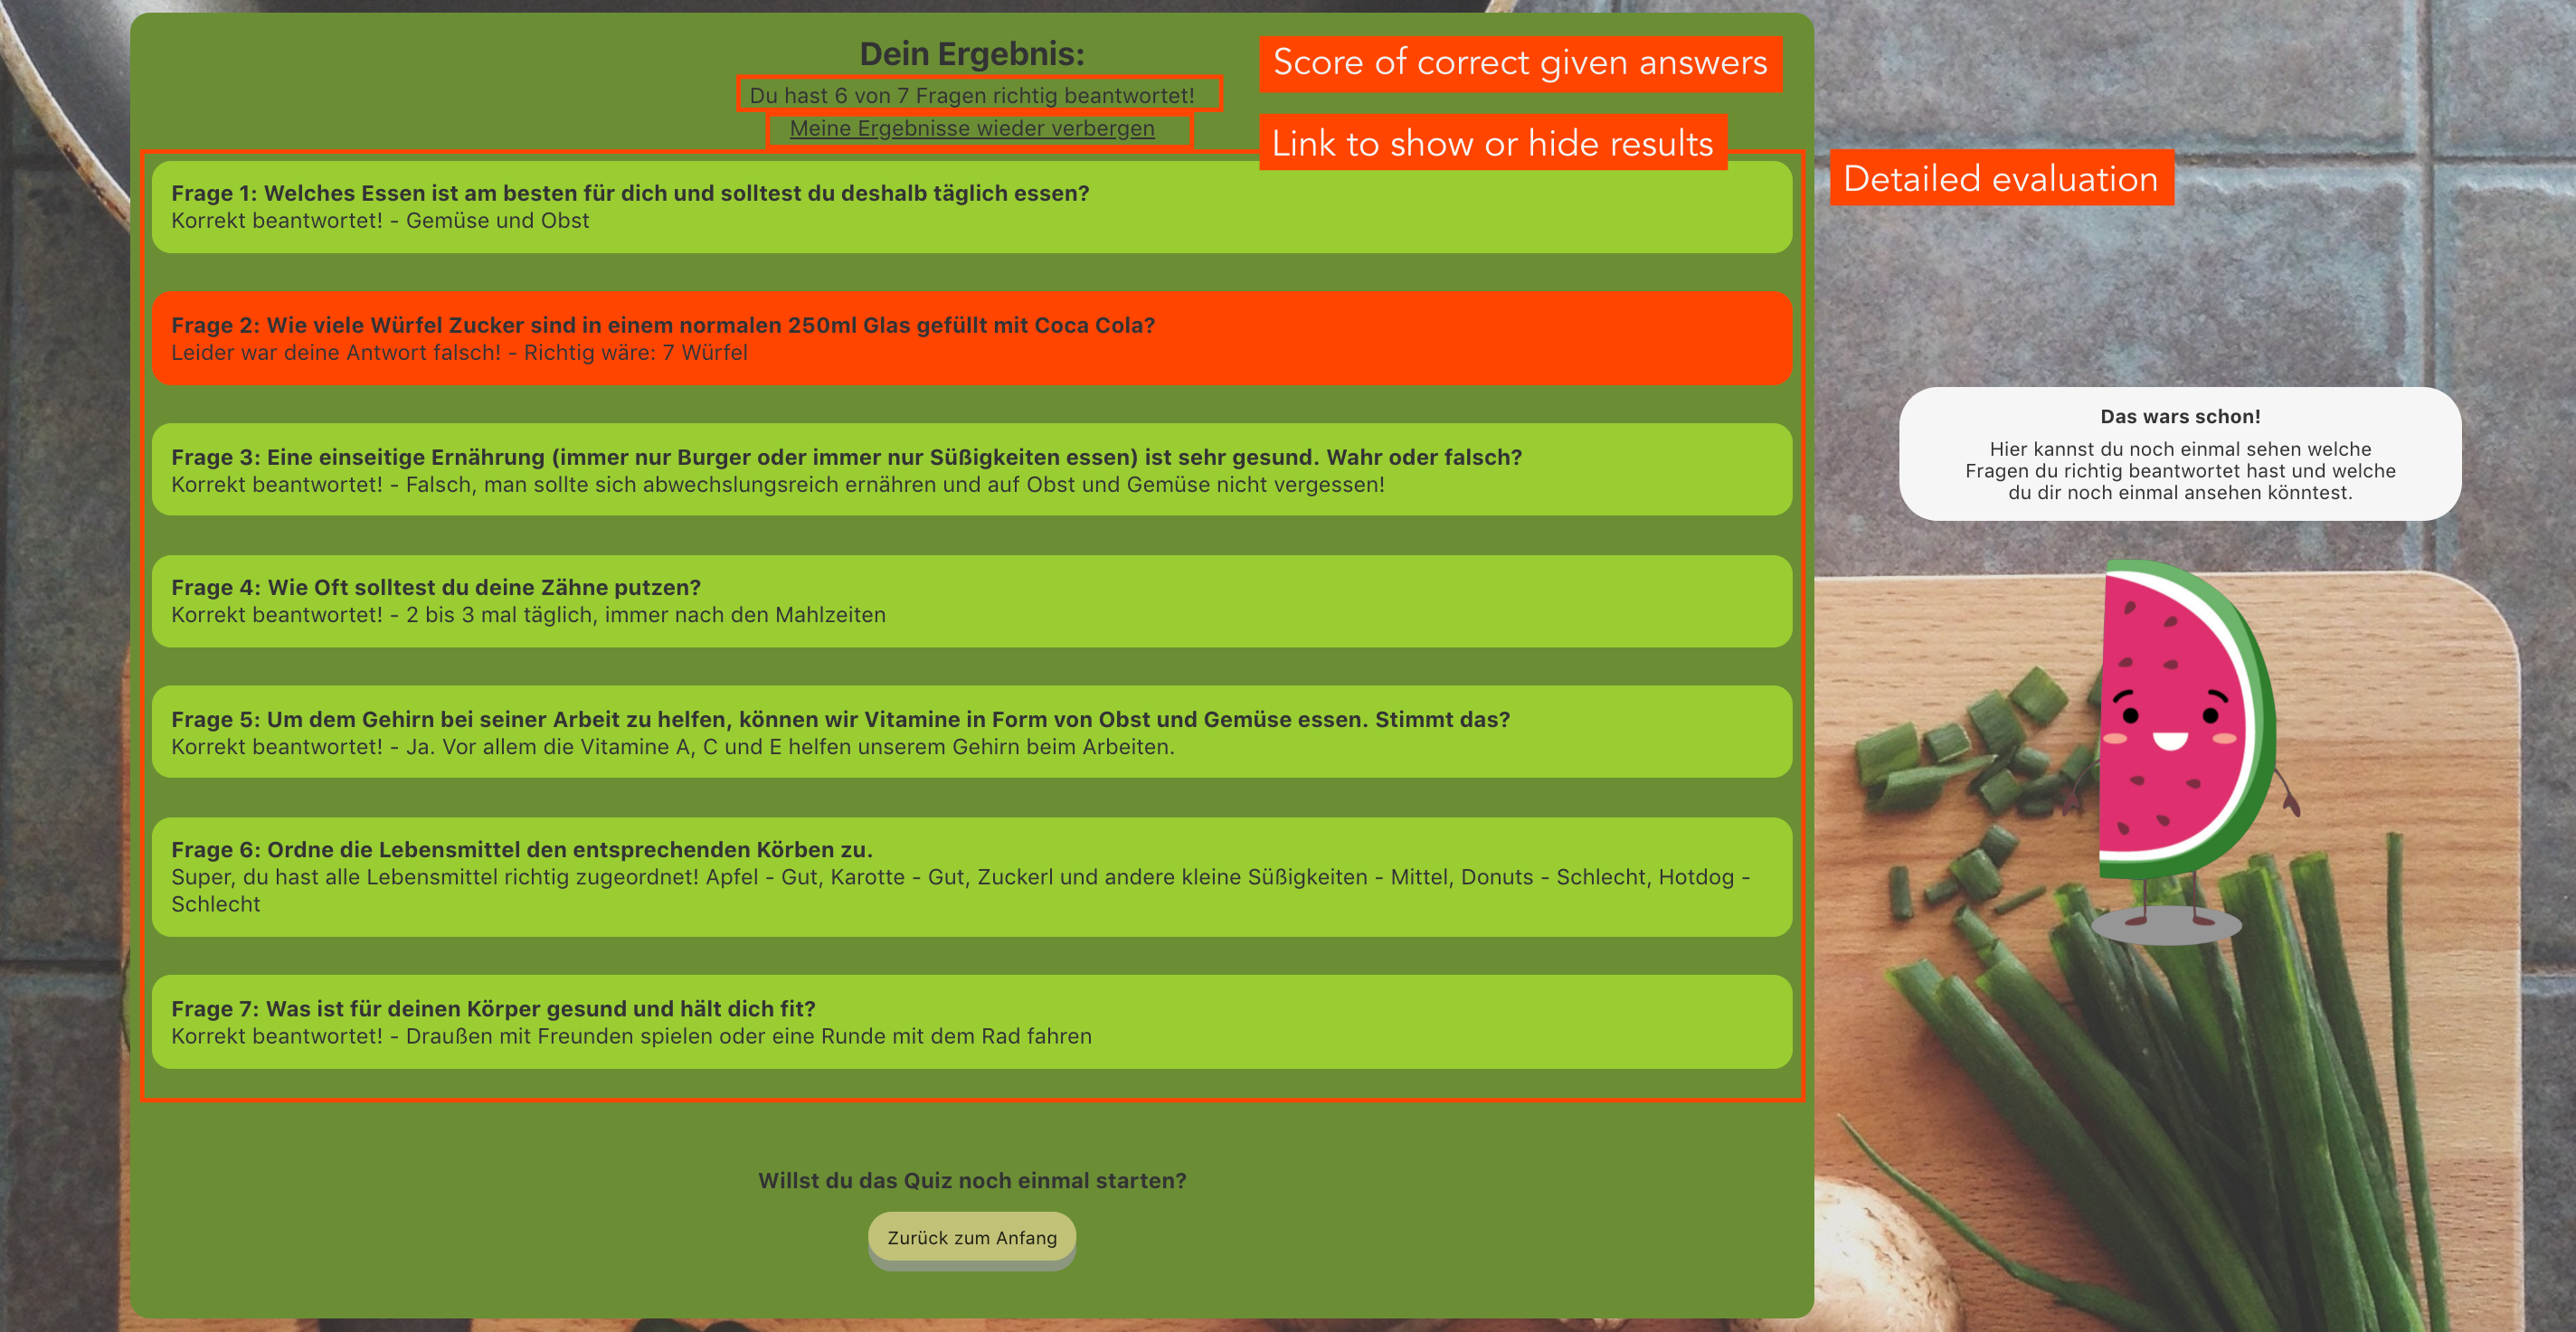
\includegraphics[width=1 \linewidth]{images/evaluation.png}
    \caption{
        Evaluation screen for the results of the quiz
    }
    \label{figure:Evaluation}
\end{figure}

Finally, there is also a progress bar below the helper that helps the children ascertain how far in the quiz they already are (see Figure \ref{subfigure:HelperWarning}). The progress bar supports the shorter attention span of children in comparison to adults.

\subsubsection{Difficulties and problems while implementing the prototype}
The designing and programming process of the prototype took place over the course of two and a half weeks. The elected programming language was JavaScript, and as a consequence, the chosen framework for this prototype was React. This quiz application, including seven questions about health literacy, was built from scratch and only required one developer. 
Since there was no data being collected, e.g., personally identifiable information about the residence, origin, or ethnic background of the children, the prototype did not need any backend application. Furthermore, there was no registration process that the children had to go through by entering their names, gender, et cetera. \textcite{alhussayen2015evaluating} also detected troubles with their registration process in their study, which supported the decision to exclude it in this study. Therefore, the children would not be hindered to enjoy freshening up their expertise about health literacy fully.\\
One problem that occurred throughout the development stage was the length reduction of the quiz. Since at the beginning of the programming process, it was assumed that there was more time to test the application, it was designed to contain a bigger selection of questions. Therefore, it was initially planned to present ten or more various questions from the compilation of questions. However, the length of the quiz had to be shortened last minute to further adjust the application to the abilities and needs of ten-year-olds. Furthermore, there were always presented the same seven questions during the testing. Consequently, the study can provide more accurate and comparable results on how much the children genuinely know about being healthy and proper nutrition. 

Apart from that, the implementation of the beverage question (see Figure \ref{subfigure:QuizCubes}) too presented some technical difficulties at first. A new external source Interact.js\footnote{https://interactjs.io/} was added into the project to make the drag and drop operation appear more fluent to the observer's eyes than the standard version. With the help of this source, the drag and drop process of the sugar cubes did not seem as chopped and somewhat smooth. 

To sum up, there was presumably not enough time to perfect this prototype thoroughly for the before expected extent. As a result, it is not suitable for daily use or viable for a broader audience. Nevertheless, for the purpose of this study and what was possible to attain in the short amount of time, the application was sufficient, and it fulfilled the purpose since the gathered knowledge from various previous studies was successfully integrated.

\subsection{Testing}
\label{subsection:Testing}
To test and verify the beforehand collected theoretical data, the prototype which was solely created for this thesis underwent a user testing study. Since the main target group for the application is school children, the user testing took place in an elementary school in Salzburg - Austria. All participants from the school class were in the fourth grade, and therefore, they were between the ages of nine and ten. Altogether, there were twenty-two children who participated in the study, of whom twelve were female and ten male (see Table \ref{table:GenderRatio}). 

\begin{table}
    \centering
    \begin{tabular}{ |c|c|c|c| } 
        \hline
        Children in total & Females & Males  \\
        \hline
        22 & 12 & 10 \\ 
        \hline
    \end{tabular}
    \caption{
        Gender distribution in the elementary class
    }
    \label{table:GenderRatio}
\end{table}

\subsubsection{Testing environment}
To avoid creating an exam situation, the children always tested the prototype in pairs at the same time on separate laptops. Since the user testing took place in the last week of school, there happened to occur some tumult during the user testing. In addition, the testing took place on a desk in front of the classroom in the hall. Moreover, throughout the testing, everybody in school had to clean up and get the school building ready for the holidays and the start of the next school year. As a result, from time to time a few students would walk through the halls carrying supplies around and therefore would seldom cause a distraction for the children who were taking the health literacy quiz at the time being. Although it was noisy at some point, the students were well put together and for the most part, did not get distracted. That was also supported by the fact that there were two separate laptops with individual computer mice set up on the table which did not reinforce interaction between the two attending children. Moreover, the table was facing a wall and thus not facing the open hall and the other children passing by.

\subsubsection{Test execution}
Over the course of one and a half hours, one student pair at a time came outside to take the quiz concurrently. Although the children tested the application at the same time, each child was operating on a separate laptop so that the second child would not impair the final quiz results from the first child. Furthermore, the independent quiz testing also encouraged the children not to cheat or copy each other's answers to the questions, which as a result would distort the results of the correctly answered questions of each child. \\
At the beginning of each pair's testing, they were told to start taking the quiz and come forward any time if they needed some help or had any comments or questions about the content of the quiz.
On the one hand, the majority of the children did not need any help or had any questions. On the other hand, some children had a few questions and directly asked for help. Most of the children that asked had trouble understanding or executing the question about the beverage, where they had to drag the correct amount of sugar cubes into the answer area.\\
Apart from that, some children were either too shy or too afraid to ask for help themselves. These children tended to look over to their colleague's screen to copy their answer, or plainly started talking to their friend about what to do about their problem. These children were then immediately offered help to continue completing the quiz without any struggles.\\
Apart from the need to seek help, the testing itself went along relatively smoothly. Each child needed about five and a half minutes on average to complete the whole quiz and process the acquired results. After the children looked at their own scores, they were asked a few quick questions. These questions had the purpose of collecting their thoughts and opinions about the questions of the quiz, the content as well as the whole experience of the user testing itself.
\begin{itemize}
    \item[(a)] Did you understand everything in this quiz? Were there any difficulties?
    \item[(b)] After taking this quiz, do you prefer taking a quiz on a computer or on paper?
    \item[(c)] Did you enjoy taking this quiz?
    \item[(d)] Is there anything you want to change?
\end{itemize}
The interview after the user testing only took about one and a half minutes on average because not all children were too talkative. Although almost every child replied to all the questions, some children still were too shy and did not talk much when asked the questions listed above. Nevertheless, almost everything from the feedback was positive. On the one hand, a possible reason for that is that the children were either too shy or did not have the courage to criticize the application directly. In addition, this would imply that they would not have the safety of being anonymous, because everything they expressed could be directly pinpointed back to them later on. Another possible reason could be that they did not test the application in their usual environment in class. As \textcite{walker2000screen} remarked, the students in their study were observed in their accustomed vicinity, which led to more honest comments and less pressure in general. 
Apart from this, the testing went well, and all children enjoyed participating in the user testing of this study.

As additional scrutiny of the knowledge about health literacy the children established through the quiz, there was a basket with food placed on the desk behind the laptops. This basket contained six apples and twenty-two small gummy bear packets, so every child could have something to take with them. After taking the quiz and answering the questions they were asked afterward, the children were then told to take one item from the basket as they please.
All children that were explicitly told that they could have the gummy bears did not ask if they were allowed to take the apple instead. However, if they were offered a choice, they took a moment to decide which item to take with them. The majority still took the gummy bears, but five children choose to grab the apple alternatively. Only one child did explicitly ask permission to take an apple instead of the gummy bears. Apart from the uncertain knowledge of health literacy, this part of the testing also confirmed that children were too shy to ask questions or give negative feedback directly.

\subsection{Analyzing and evaluating the results}
\label{subsection:AnalyzingResults}
In the course of this study, there were a few new findings and promising outcomes. 
The goal of this study was to create an interface that is optimally suited for children. Furthermore, the designed interface should educate students in primary school about health literacy and improve their knowledge about nutrition and health in general. For that reason, all scores of the quiz have been collected. This documentation was made to see how much they already know and hence, how familiar they already are with proper health literacy at an early age.\\
As a consequence, the following sections will evaluate further outcomes from the user testing and specify improvements that would be necessary to perfect the prototype and make it suitable for school classes.

\subsubsection{Results from the quiz and interview}
As displayed in Figure \ref{figure:CorrAnswers}, none of the twenty-two children achieved a score of zero, one or two. Therefore, all children answered at least three questions from the health literacy quiz correctly. Most often, five questions were correctly answered. Only two children were able to answer all seven questions without making a mistake. Besides, both of these children turned out to be female. Furthermore, two of the three children who gave six correct answers were also female. These results imply that the females of this class are better acquainted with health literacy in general.\\
Apart from that, most mistakes were made while answering question two and six. These questions were more complicated than only choosing and clicking one answer, e.g., multiple-choice and true or false. For example, for the second quiz question, the children had to pull sugar cubes into an answering field. The sixth question required the children to categorize the food based on how healthy those particular items are. 
\begin{figure}[!ht]
    \centering
    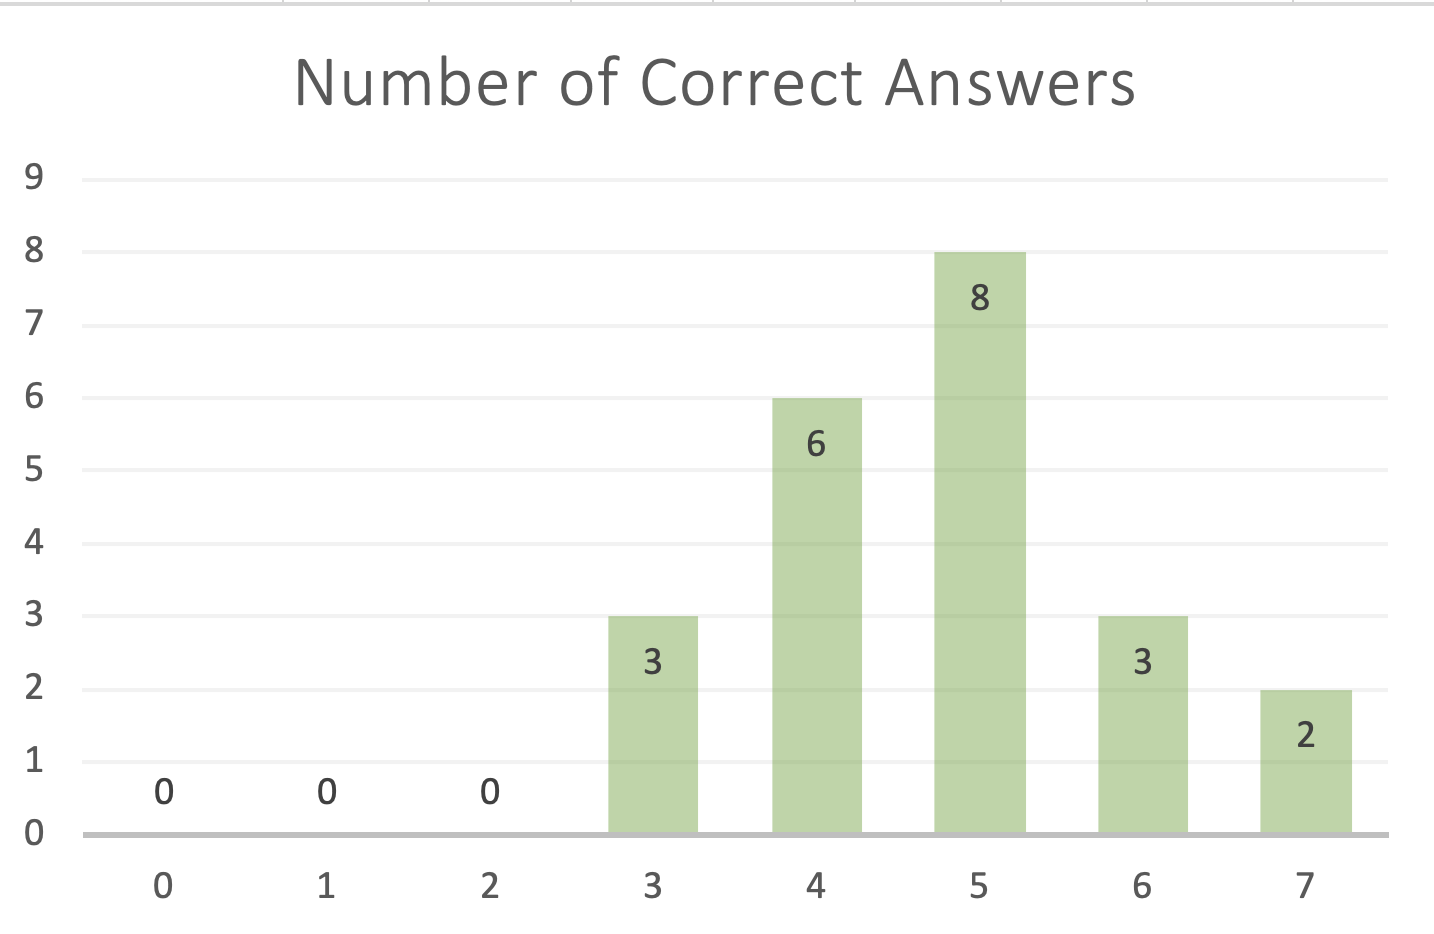
\includegraphics[width=1 \linewidth]{images/num_corr_answers.png}
    \caption{
        Distribution of correct given answers of all children
    }
    \label{figure:CorrAnswers}
\end{figure}

Moreover, almost all students understood the formulation of the questions, and for the most part, knew how to navigate through the quiz.
Although a button needs to be pressed at the beginning of the quiz to start (see Figure \ref{figure:QuizHome}), not all students were able to understand that. Two students were too eager to start and did not read the instructions either. As a result, they first tried to click on the helper and the bubble above to start the quiz, before they identified the start button correctly. Apart from that mishap, the guidance figure was received well by the children.
Aside from that, the second question of the quiz about the beverage (see Figure \ref{subfigure:QuizCubes}) has constituted an exception. To answer the question correctly, the children had the task of dragging the correct number of sugar cubes into the grey answer field. Various students did not know how to complete this exercise and hence asked for help. Furthermore, they also complained about physical difficulties while dragging the cubes with the touchpad of the laptop. Consequently, they had to fall back on the computer mouse. One boy did not understand the given instructions at all and pulled the sugar cubes into the image of the soda glass (see image below the question in Figure \ref{subfigure:QuizCubes}). 
Moreover, a few children also vocalized their disagreement with the answer to this question. They claimed to know the correct sugar amount but then realized the question referred to a different kind of vessel and therefore, a different sugar ratio. \\
The sixth question from the quiz, where the children needed to place the foods in the matching categories, also caused some technical difficulties and confusion for the students. After the children clicked the button that displays the immediate evaluation, the food items were still draggable. As a result, three children thought they could correct their mistakes instantly and were left confused when they could not mend their error but got redirected to next question. Consequently, it had to be explained to them that mending their mistakes was not possible. To gain a better score, they would have to take the quiz once more.

The interview afterward adduced mainly consistent results. Almost every child liked the quiz application and voiced their enjoyment. Moreover, all students disclosed that they had much fun. Besides, some children implied similarities to a game because of the score at the end.
When they were asked if they prefer digitized quizzes instead of hard-copy tests, all children said that would rather do a quiz on the computer. One student mentioned that they want to have tablets in school instead of regular books so that they would have fewer appliances to carry to school every day. Another student explained that they preferred this quiz because they did not have to cogitate as much while answering the multiple-choice questions. Furthermore, they said that on paper, they need to think of elaborate answers and write more instead of only clicking buttons. Aside from that, all children were mostly satisfied with the interface.\\
As mentioned before, a couple of students were too shy to answer any questions at all in the interview. One possible reason for that is that they were not in their usual environment and therefore, did not feel relaxed enough to speak up. As a result, all the feedback was positive, and no one criticized anything significant. Nevertheless, one child expressed their wish to include only questions like question six, where the food had to be categorized. 

\subsubsection{Testing environment and implementation of the prototype}
The testing of the application had to be done in the last week of school due to time constraints. As a result, the conditions for a perfect environment were not ideal. Therefore, some result could have been influenced by that condition. Furthermore, it would have been better if there were multiple user tests carried out to develop and improve the prototype additionally. Consequently, the testing environment should be adapted, and the user testing should take place in a separate and quiet room. It would guarantee fewer distractions, for example, children running around in the hall and attempts of intervening.\\
Moreover, it should be considered to conduct the user testing only with one child at a time. Individual testing would reduce the possibility of external influences or copying answers. As a result, it would deliver a clean result of solely one child's knowledge. Nonetheless, some children could experience disadvantages because they were too shy to ask for help directly and talked to their peer instead.\\
Although all feedback was positive, there could have been children that had some criticism but did not dare to speak up. A separate rating and feedback system should be employed to avoid this in further testing. Consequently, it would ensure more honest feedback. A possible approach for that was introduced by \textcite{alhussayen2015evaluating} where children could give feedback in the form of smileys that show whether or not they like the application.

Furthermore, some programming issues need to be fixed, and some ideas could get implemented additionally in the future. Question six includes one bug that needs to be corrected in order to ensure proper usage. When the instant evaluation is displayed, the food items need to be prohibited from being draggable. Therefore, no children get confused and think they can immediately correct their answer. \\
Besides, the answers to the questions should not be placed in the same order every time. Consequently, when a child is playing the quiz a second time, it could memorize the spot the correct answer is placed in instead of memorizing the content of the correct answer.
Hence, the answers should be shuffled before they get arranged on the screen.\\
To address multiple senses, it should be considered to integrate acoustic feedback into the application. For example, if a child answers a question correctly, a correlating sound could be played to intensify the success.
Moreover, the incorporation of various level of difficulties is a possible way to expand the application. Since some children complaint about too simple questions adding a different difficulty level would support that children have different amounts of knowledge about health literacy.

\section{Discussion}
\label{section:Discussion}
In the course of this study, a quiz application was developed with the intention of being very engaging, appealing, and most importantly, suitable for children. All included features were based on the beforehand researched theoretical data. Although the prototype was not ideally perfected and is not ready to be introduced to a broader audience or integrated into the classroom at the current stage, it turns out to be a success overall. All twenty-two students who participated in the study enjoyed the quiz and had fun answering all the questions. Moreover, the children appreciated the guidance character, as in the study of \textcite{gossen2012search} and the variety of different questions. They also enjoyed that the approach of playfully learning new information instead of only reading about it in books which confirms prior research like the studies from \textcite{gossen2012search, boyd2015evaluating}.\\
Furthermore, they were accustomed to health literacy and especially proper nutrition before this testing since most of the children accomplished an adequate score by answering most of the questions correctly. This is a positive outcome since it is vital to learn about health literacy as soon as possible \autocite{velardo2017emphasizing}. \\
Nevertheless, apart from the positive feedback that the quiz application received, the real opinions of the children could have been affected by their shyness or feeling of being unable to talk freely about their opinion. This could be avoided by launching a separate feedback system, similar to the system from \textcite{alhussayen2015evaluating}, to ensure anonymity for the children. 

\section{Conclusion}
\label{section:Conclusion}
The aim of this thesis was to develop an interface with information about health literacy that is especially appealing and satisfying for the needs and abilities of children. 
For this reason, a web-based quiz application about health literacy was developed. The focus of the content was on nutrition since it is a part of our daily lives, and hence, children are very familiar with it. To create an optimal application for children, this thesis explored different approaches of already existing applications that were made for children \autocite{gossen2012search, alhussayen2015evaluating, adattil2018effects}. Furthermore, the reasons as to why children need different attributes in interfaces were collected and considered during the designing process.

During the testing, it became apparent that children nowadays are principally already in close contact with health literacy, especially nutrition. This finding is supported by the fact that none of the children scored two or less correct answers. Nevertheless, some external factors during the user testing process may have influenced the scores. Consequently, to get even more accurate and more adequate results, future user testing on this application needs to be done in a better testing environment.\\
Besides, to make the current prototype more suitable for classrooms or broader audiences, more user testings and additionally, more constructive feedback from the children is necessary. Furthermore, this study showed that not all children are at the same level of knowledge when it comes to health literacy. As a result, different difficulty levels for the quiz should be considered for further development of the application.